\chapter{Metodología}

Se necesitan 4 pasos para poder cumplir los objetivos y crear una infraestructura de red funcional, que permita la ejecución de múltiples consultas, manejo de datos y el desarrollo de la aplicación.

\begin{enumerate}
    \item Levantado de un sistema operativo y una VPN que permita el acceso a los servidores, permitiendo un mejor ambiente de trabajo.
    \item Desarrollar arquitectura de base de datos para gestionar los datos, asegurando la seguridad de los mismos.
    \item Implementar un módulo de APIs para bases de datos que permita consultas e inserciones.
    \item APIs para acceder a los diferentes modelos para uso interno y externo, que permitan el envío y recepción de información entre los módulos. Al igual que la arquitectura de red y de sistema para que el proceso sea lo más eficiente posible.
\end{enumerate}

\section{Levantamiento de un sistema operativo y configuración de VPN}

Para garantizar un ambiente de trabajo seguro y eficiente, se ha implementado Ubuntu 22.08 como sistema operativo en un servidor Dell R740. Se elimino el controlador RAID para liberar un disco duro de 1.92T, adecuándolo para las necesidades del proyecto. Además, se configuró una VPN utilizando OpenVPN, lo cual permite un acceso directo y seguro a los servidores. La configuración de la VPN se complementó con ajustes en los firewalls institucionales otorgados por la universidad, facilitando el acceso remoto y el manejo del servidor desde múltiples dispositivos sin comprometer la seguridad. Esta configuración permite una administración centralizada y segura del servidor, asegurando que solo usuarios autorizados puedan acceder a los recursos críticos del sistema.

\begin{figure}[H]
    \centering
    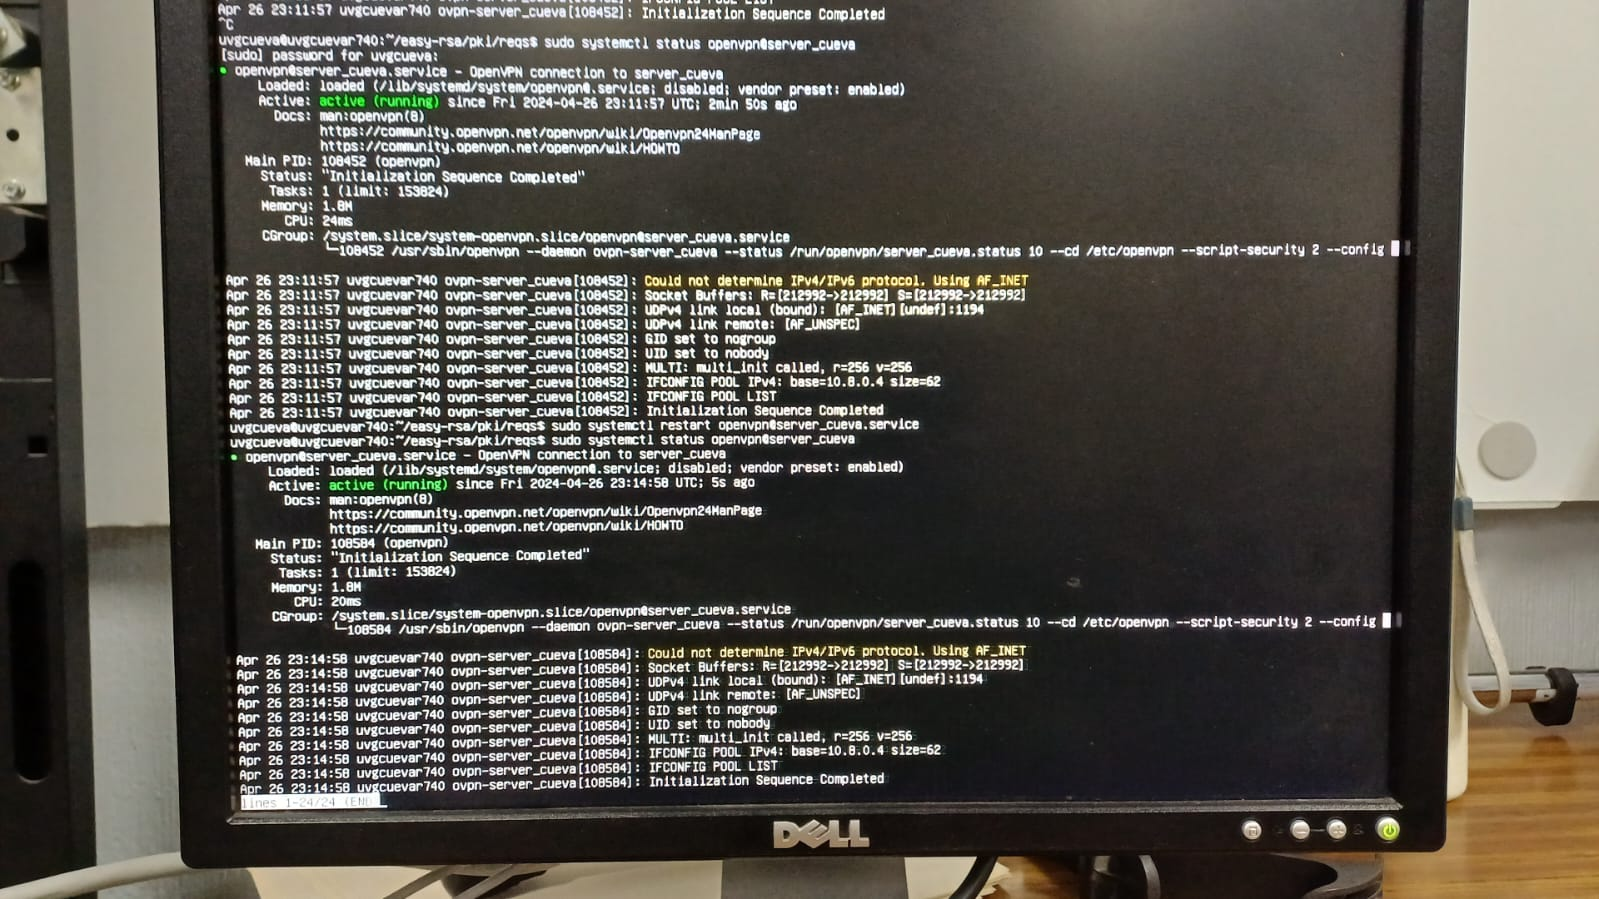
\includegraphics[width=0.7\textwidth]{figuras/LevantadoOpenVPN.png}
    \caption{LevantadoOpenVPN.}
    \label{fig:LevantadoOpenVPN}
\end{figure}
Como se puede observar en la Figura \ref{fig:LevantadoOpenVPN}, la máquina virtual ha sido levantada correctamente.

\begin{figure}[H]
    \centering
    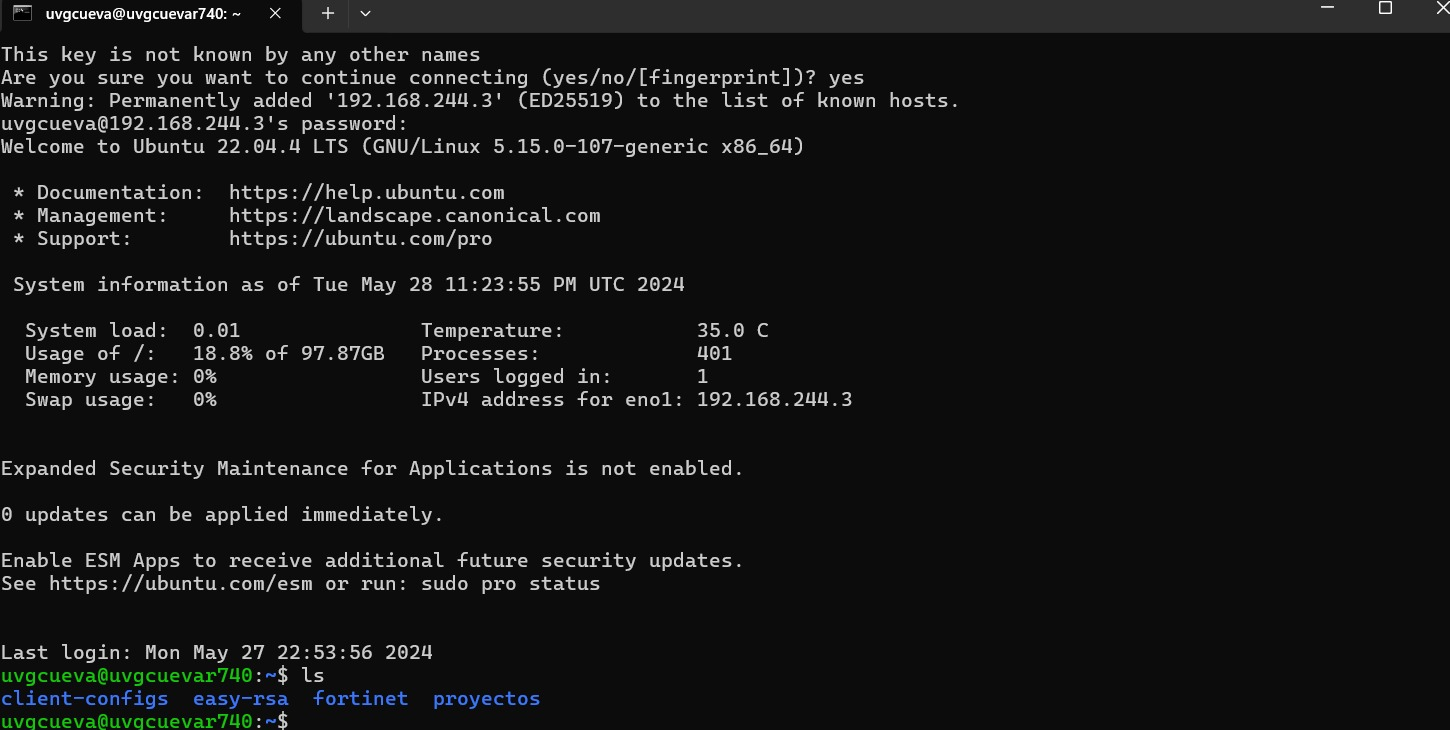
\includegraphics[width=0.7\textwidth]{figuras/ConexionSSH.png}
    \caption{ConexionSSH.}
    \label{fig:ConexionSSH}
\end{figure}
Además, en la Figura \ref{fig:ConexionSSH} se muestra la conexión generada con la VPN mediante SSH.


El proceso requiere conectarse a través de la infraestructura de red de la universidad y la VLAN específica donde se encuentra el rack y el servidor. Para lograr esto, se utiliza FortiClient VPN, que proporciona una conexión segura y cifrada directamente a la VLAN donde se encuentra el servidor. Para acceder a la VPN, se necesita un archivo de configuración .ovpn que se utiliza con OpenVPN. Una vez conectado a la VPN, se puede acceder al servidor de manera segura mediante SSH. Esto se realiza abriendo una terminal y utilizando el comando ssh uvgcueva@192.168.244.3 con las credenciales correspondientes. Este método asegura que la administración remota de las máquinas virtuales se realice de manera eficiente y segura, permitiendo a los usuarios realizar tareas administrativas y de mantenimiento sin estar físicamente presentes en el sitio.

\section{Desarrollo de la arquitectura de base de datos}

Se ha seleccionado PostgreSQL para gestionar la base de datos relacional del proyecto debido a su robustez y eficacia en el manejo de grandes volúmenes de datos, incluyendo datos de usuarios, videos y otros tipos de información. PostgreSQL ofrece avanzadas características de seguridad que son esenciales para proteger los datos contra accesos no autorizados. Su arquitectura permite realizar operaciones complejas de base de datos de manera eficiente, asegurando la integridad y la privacidad de los datos gestionados. En la arquitectura se hace especial hincapié en la importancia de diseñar con flexibilidad, utilizando estándares que permitan la interacción entre diferentes sistemas y tecnologías.

Para implementar PostgreSQL en nuestro proyecto de forma efectiva y segura, seguiremos una metodología estructurada que abarcará desde la planificación inicial hasta la integración con otros sistemas. Comenzaremos evaluando los requisitos de hardware y software para seleccionar la versión óptima de PostgreSQL y preparar el entorno del sistema operativo. Una vez instalado PostgreSQL, procederemos a configurar los parámetros de rendimiento y seguridad, como la memoria, conexiones permitidas, y configuraciones de cifrado, además de establecer un protocolo regular de mantenimiento que incluirá actualizaciones y parches.

La seguridad será una prioridad, implementando roles y permisos detallados para controlar el acceso a los datos y asegurar todas las comunicaciones mediante SSL/TLS. Paralelamente, desarrollaremos y configuraremos procesos de ETL para automatizar la extracción, transformación y carga de datos, asegurando la integridad y utilidad de la información gestionada. Además, diseñaremos y desarrollaremos APIs que permitan una interacción segura y eficiente con otras aplicaciones, implementando mecanismos robustos de autenticación y autorización.

Finalmente, estableceremos sistemas de monitoreo para supervisar constantemente el rendimiento y la seguridad de la base de datos y las APIs, permitiendo ajustes continuos para optimizar la configuración según las necesidades cambiantes del proyecto. Este enfoque metodológico asegura no solo la implementación técnica efectiva de PostgreSQL, sino también el mantenimiento de un sistema seguro, eficiente y adaptable a largo plazo.

% Cuadros de la base de datos
% ---------------------------

% Tabla: user
\begin{table}[H]
\centering
\begin{tabularx}{\textwidth}{|l|l|l|X|}
\hline
\textbf{Nombre del campo} & \textbf{Tipo de dato} & \textbf{Restricciones} & \textbf{Descripción} \\ \hline
id                       & Integer               & Primary Key            & Identificador único del usuario. \\ \hline
mail                     & String(120)           & Unique, Not Null       & Correo electrónico del usuario. \\ \hline
password                 & String(120)           & Not Null               & Contraseña del usuario. \\ \hline
streak                   & Integer               & Default = 0            & Puntuación o racha del usuario. \\ \hline
quetzalito               & String                & Nullable               & Color de la imagen de perfil. \\ \hline
confirmed                & Boolean               & Default=False          & Indica si el usuario ha confirmado su cuenta. \\ \hline
\texttt{last\_streak\_update} & DateTime            & Default=datetime.utcnow & Indica la última hora que se agregó un streak. \\ \hline
\end{tabularx}
\caption{Tabla: user}
\end{table}

% Tabla: video
\begin{table}[H]
\centering
\begin{tabularx}{\textwidth}{|l|l|l|X|}
\hline
\textbf{Nombre del campo} & \textbf{Tipo de dato} & \textbf{Restricciones} & \textbf{Descripción} \\ \hline
id                       & Integer               & Primary Key            & Identificador único del video. \\ \hline
id\_user                 & Integer               & ForeignKey(user.id), Not Null & Referencia al usuario que subió el video. \\ \hline
traduction\_esp          & String(255)           & Nullable                & Traducción del video al español. \\ \hline
sentence\_lensegua       & String(255)           & Not Null                & Oración en lengua de señas guatemalteca. \\ \hline
video                    & String(255)           & Not Null                & Ruta del archivo de video. \\ \hline
prev\_image              & String(255)           & Nullable                & Imagen previa del video. \\ \hline
is\_favorite             & Boolean               & Default=False           & Indica si el video es favorito del usuario. \\ \hline
\end{tabularx}
\caption{Tabla: video}
\end{table}

% Tabla: traducción
\begin{table}[H]
\centering
\begin{tabularx}{\textwidth}{|l|l|l|X|}
\hline
\textbf{Nombre del campo} & \textbf{Tipo de dato} & \textbf{Restricciones} & \textbf{Descripción} \\ \hline
id                       & Integer               & Primary Key            & Identificador único de la traducción. \\ \hline
id\_user                 & Integer               & ForeignKey(user.id), Not Null & Referencia al usuario que hizo la traducción. \\ \hline
sentence\_lensegua       & String(255)           & Not Null                & Oración en lengua de señas guatemalteca. \\ \hline
traduction\_esp          & String(255)           & Nullable                & Traducción al español. \\ \hline
is\_favorite             & Boolean               & Default=False           & Indica si la traducción es favorita. \\ \hline
\end{tabularx}
\caption{Tabla: traducción}
\end{table}

% Tabla: dictionary
\begin{table}[H]
\centering
\begin{tabularx}{\textwidth}{|l|l|l|X|}
\hline
\textbf{Nombre del campo} & \textbf{Tipo de dato} & \textbf{Restricciones} & \textbf{Descripción} \\ \hline
id                       & Integer               & Primary Key            & Identificador único del diccionario. \\ \hline
id\_user                 & Integer               & ForeignKey(user.id), Not Null & Referencia al usuario. \\ \hline
id\_word                 & String(255)           & Not Null                & Palabra o identificador del término en el diccionario. \\ \hline
\end{tabularx}
\caption{Tabla: dictionary}
\end{table}

El diagrama de entidad-relación presentado en la Figura \ref{fig:entidad_relacion} muestra la estructura y las relaciones entre las tablas diseñadas para el proyecto. 

En este diagrama se observan las entidades principales del sistema: \texttt{user}, \texttt{video}, \texttt{traducción} y \texttt{dictionary}. Cada una de estas entidades incluye atributos que definen su propósito dentro del sistema. Por ejemplo, la tabla \texttt{user} almacena información esencial del usuario como su correo, contraseña y estado de confirmación, mientras que la tabla \texttt{video} registra información de los videos asociados a los usuarios, incluyendo traducciones y metadatos adicionales.

Las relaciones entre las entidades destacan cómo interactúan entre sí. Por ejemplo, la tabla \texttt{video} está vinculada a la tabla \texttt{user} mediante una relación de uno a muchos (\texttt{1:N}), lo que indica que cada usuario puede tener múltiples videos asociados. Asimismo, la tabla \texttt{traducción} permite almacenar traducciones específicas realizadas por los usuarios, vinculándose también a través de una relación de \texttt{1:N} con \texttt{user}.

Este diseño garantiza la flexibilidad y escalabilidad del sistema, permitiendo el manejo eficiente de los datos necesarios para cumplir con los objetivos del proyecto.

\begin{figure}[H]
    \centering
    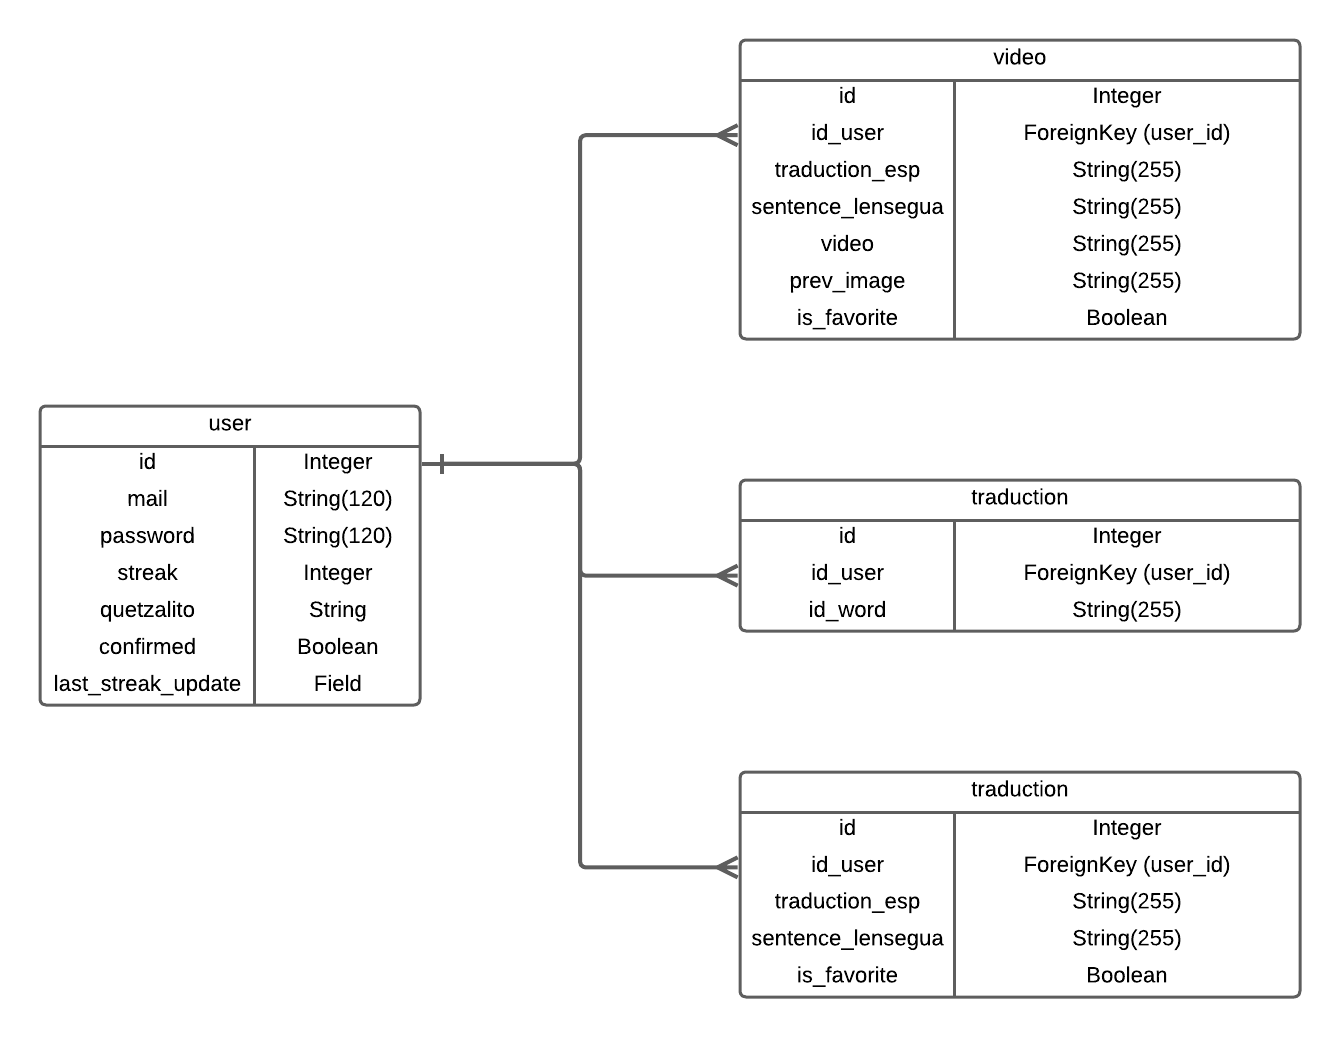
\includegraphics[width=0.5\textwidth]{figuras/entidad_relacion.png}
    \caption{Diagrama entidad relación.}
    \label{fig:entidad_relacion}
\end{figure}

% Fin de cuadros de la base de datos
% ---------------------------

\section{Implementacion de API's}

Para facilitar las consultas y las inserciones de datos, se utilizará Flask como framework principal debido a su ligereza y capacidad para manejar peticiones de manera eficiente. Este módulo API permitirá un manejo flexible de diferentes formatos de datos, incluyendo videos y texto. La estructura del módulo está diseñada para optimizar el rendimiento del sistema, minimizando el uso de recursos y maximizando la velocidad de respuesta, lo que es crucial para procesar y responder a las interacciones de los usuarios en tiempo real.

% Definir colores personalizados para las filas
\definecolor{lightgreen}{RGB}{199,233,192}
\definecolor{lightblue}{RGB}{180,220,240}
\definecolor{lightred}{RGB}{252,205,205}

% Tabla para las APIS
% -------------------

% Tabla de user_routes
\begin{table}[H]
\centering
\begin{tabularx}{\textwidth}{|l|l|l|X|}
\hline
\textbf{Nombre} & \textbf{TIPO} & \textbf{Entrada} & \textbf{Salida} \\ \hline
login & POST & email, password & id\_user \\ \hline
signup & POST & email, password, quetzalito & id\_user \\ \hline
forgot\_password & POST & email & 200-OK \\ \hline
change\_password & POST & id\_user, new\_password & id\_user, 200-OK \\ \hline
\end{tabularx}
\caption{Resumen de Rutas de API: \texttt{user\_routes}}
\label{tab:user_routes}
\end{table}

% Tabla de video_routes
\renewcommand{\arraystretch}{1.3} % Aumenta la altura de las filas
\begin{table}[H]
\centering
\begin{tabularx}{\textwidth}{|l|l|X|X|}
\hline
\textbf{Nombre} & \textbf{TIPO} & \textbf{Entrada} & \textbf{Salida} \\ \hline
send\_video & POST & id\_user, video & id\_video, traduction\_lensegua, traduction\_esp \\ \hline
report\_video & POST & id\_user, id\_video, report\_message, report\_img (png) & 200-OK \\ \hline
fav\_video & POST & id\_user, id\_video, prev\_video (png) & 200-OK \\ \hline
remove\_video & DELETE & id\_video & 200-OK \\ \hline
remove\_fav\_video & POST & id\_user, id\_video & 200-OK \\ \hline
download\_video & POST & route\_video & ruta\_video \\ \hline
download\_images & POST & route\_image & ruta\_image \\ \hline
\end{tabularx}
\caption{Resumen de Rutas de API: \texttt{video\_routes}}
\label{tab:video_routes}
\end{table}

% Tabla de traduction_routes
\begin{table}[H]
\centering
\begin{tabularx}{\textwidth}{|l|l|l|X|}
\hline
\rowcolor{blue!30} \textbf{Nombre} & \textbf{TIPO} & \textbf{Entrada} & \textbf{Salida} \\ \hline
send\_traduction & POST & id\_user, sentence\_lensegua & id\_sentence, traduction\_esp \\ \hline
fav\_traduction & POST & id\_user, id\_sentence & 200-OK \\ \hline
remove\_traduction & DELETE & id\_sentence & 200-OK \\ \hline
remove\_fav\_traduction & POST & id\_user, id\_sentence & 200-OK \\ \hline
\end{tabularx}
\caption{Resumen de Rutas de API: traduction\_routes}
\label{tab:traduction_routes}
\end{table}

% Tabla de dictionary_routes
\begin{table}[H]
\centering
\begin{tabularx}{\textwidth}{|l|l|l|X|}
\hline
\textbf{Nombre} & \textbf{TIPO} & \textbf{Entrada} & \textbf{Salida} \\ \hline
add\_dictionary & POST & id\_user, id\_word & 200-OK \\ \hline
remove\_dictionary & DELETE & id\_user, id\_word & 200-OK \\ \hline
get\_dictionary & POST & id\_user & palabras (json) \\ \hline
\end{tabularx}
\caption{Resumen de Rutas de API: \texttt{dictionary\_routes}}
\label{tab:dictionary_routes}
\end{table}

% Tabla de profile_routes
\begin{table}[H]
\centering
\begin{tabularx}{\textwidth}{|l|l|l|X|}
\hline
\textbf{Nombre} & \textbf{TIPO} & \textbf{Entrada} & \textbf{Salida} \\ \hline
get\_user\_info & POST & id\_user & email, streak, quetzalito, videos\_fav (json), traductions\_fav (json) \\ \hline
get\_video & POST & id\_user, id\_video & video (mp4) \\ \hline
get\_image & POST & id\_user, id\_video & image (png) \\ \hline
delete\_user & DELETE & id\_user & 200-OK \\ \hline
add\_streak & POST & id\_user & 200-OK \\ \hline
remove\_streak & POST & id\_user & 200-OK \\ \hline
\end{tabularx}
\caption{Resumen de Rutas de API: \texttt{profile\_routes}}
\label{tab:profile_routes}
\end{table}

% Tabla de mail_routes
\begin{table}[H]
\centering
\begin{tabularx}{\textwidth}{|l|l|l|X|}
\hline
\textbf{Nombre} & \textbf{TIPO} & \textbf{Entrada} & \textbf{Salida} \\ \hline
confirm & POST & email & 200-OK \\ \hline
\end{tabularx}
\caption{Resumen de Rutas de API: \texttt{mail\_routes}}
\label{tab:mail_routes}
\end{table}


% Fin de las tablas para APIS
% ---------------------------
% AQUI: meter la imagen de resultadosDeLlamarUsandoSQLAlchemy

\subsection{Flujo de trabajo para sistema de apis}

La infraestructura del sistema sigue un flujo bien definido en el manejo de solicitudes y respuestas, diseñado para garantizar un equilibrio entre eficiencia y robustez.

\begin{enumerate}
    \item \textbf{Cliente envía una solicitud:} 
    El punto de partida se da cuando un cliente realiza una solicitud HTTP al servidor, por ejemplo, \texttt{mi-ip:4242/example}. Este podría ser un navegador web, una aplicación móvil, o cualquier sistema que consuma las APIs que estamos desarrollando. En este primer punto, la solicitud se envía al servidor en la ruta definida.

    \item \textbf{Nginx recibe la solicitud:} 
    Nginx actúa como la primera línea de defensa y como un proxy inverso. Es el encargado de recibir todas las solicitudes entrantes y decidir cómo deben ser manejadas. Nginx no solo se encarga de redirigir las solicitudes, sino que también es clave en el manejo de conexiones concurrentes, balanceo de carga y la administración de recursos estáticos si es necesario. Gracias a Nginx, el sistema puede gestionar eficientemente un alto volumen de solicitudes simultáneas, \textit{distribuyéndolas} entre los diferentes trabajadores de Gunicorn.

    \item \textbf{Nginx reenvía la solicitud a Gunicorn:} 
    Una vez que Nginx recibe la solicitud, la reenvía a Gunicorn utilizando un socket Unix o TCP, según la configuración definida. Gunicorn es un servidor de aplicaciones WSGI diseñado específicamente para ejecutar aplicaciones Flask en entornos de producción. En este paso, Gunicorn toma la solicitud y la pasa al núcleo de la aplicación Flask.

    \item \textbf{Gunicorn procesa la solicitud:} 
    Al recibir la solicitud de Nginx, Gunicorn la envía a la aplicación Flask, encargada de manejar la lógica de negocio asociada a cada \textit{endpoint}. Por ejemplo, si la solicitud se realizó a la ruta \texttt{/example}, Flask ejecutará la función asociada a esa ruta. Esta función puede incluir lógica para consultar una base de datos, realizar cálculos, o incluso comunicarse con otros servicios.

    \item \textbf{Flask genera y envía la respuesta:} 
    Una vez que Flask ha procesado la solicitud, genera una respuesta adecuada. Esta respuesta puede estar en formato JSON, HTML, o cualquier otro formato según lo requerido por el cliente. Posteriormente, Flask devuelve la respuesta a Gunicorn, que se encargará de llevarla al siguiente paso en el flujo.

    \item \textbf{Gunicorn reenvía la respuesta a Nginx:} 
    Al recibir la respuesta de Flask, Gunicorn la reenvía a Nginx, que tiene la responsabilidad de empaquetarla y prepararla para ser entregada de vuelta al cliente.

    \item \textbf{Nginx devuelve la respuesta al cliente:} 
    Finalmente, Nginx envía la respuesta al cliente que hizo la solicitud. El cliente recibe la respuesta HTTP, que puede ser procesada y presentada de acuerdo a sus necesidades. Este paso cierra el ciclo de la solicitud, asegurando que el sistema haya gestionado de manera eficiente tanto la entrada como la salida de información.
\end{enumerate}

\subsection{Diagrama de Flujo de la Arquitectura de Solicitudes}

En esta sección se presenta el diagrama de flujo de la arquitectura del proyecto (Figura \ref{fig:diagrama_flujo}), el cual ilustra cómo se gestionan las solicitudes en el sistema. Nuestra estructura sigue el principio de "dividir y conquistar", separando las múltiples solicitudes en secciones que tienen objetivos específicos y bien definidos. 

Las solicitudes se agrupan en diferentes módulos, cada uno manejado por un archivo dedicado:
\begin{itemize}
    \item \textbf{profile\_routes.py:} Gestiona operaciones relacionadas con la información del perfil del usuario, como obtener datos personales, videos y traducciones favoritas, y la gestión de la racha (\textit{streak}).
    \item \textbf{user\_routes.py:} Maneja operaciones de autenticación y registro, como iniciar sesión, registrarse, y cambiar contraseñas.
    \item \textbf{video\_routes.py:} Se ocupa de la carga, gestión y eliminación de videos, así como de marcar o desmarcar favoritos y manejar imágenes de previsualización.
    \item \textbf{traduction\_routes.py:} Administra las traducciones de frases en Lensegua al español, permitiendo marcar traducciones como favoritas o eliminarlas.
    \item \textbf{dictionary\_routes.py:} Permite agregar, eliminar y consultar palabras en el diccionario de favoritos del usuario.
    \item \textbf{mail\_routes.py:} Facilita el envío de correos electrónicos, como en el caso de restablecimiento de contraseñas.
\end{itemize}

Todos estos módulos giran en torno al uso del archivo \textbf{models.py}, el cual actúa como el eje central del sistema. Este archivo define las entidades y modelos utilizados para interactuar con la base de datos, permitiendo que todas las secciones puedan acceder y realizar operaciones en ella de manera eficiente y centralizada.

Esta división modular asegura una arquitectura organizada, fácil de mantener y escalable, donde cada módulo se encarga de tareas específicas, mientras que el modelo central proporciona una única fuente de verdad para la interacción con los datos.

\begin{figure}[H]
    \centering
    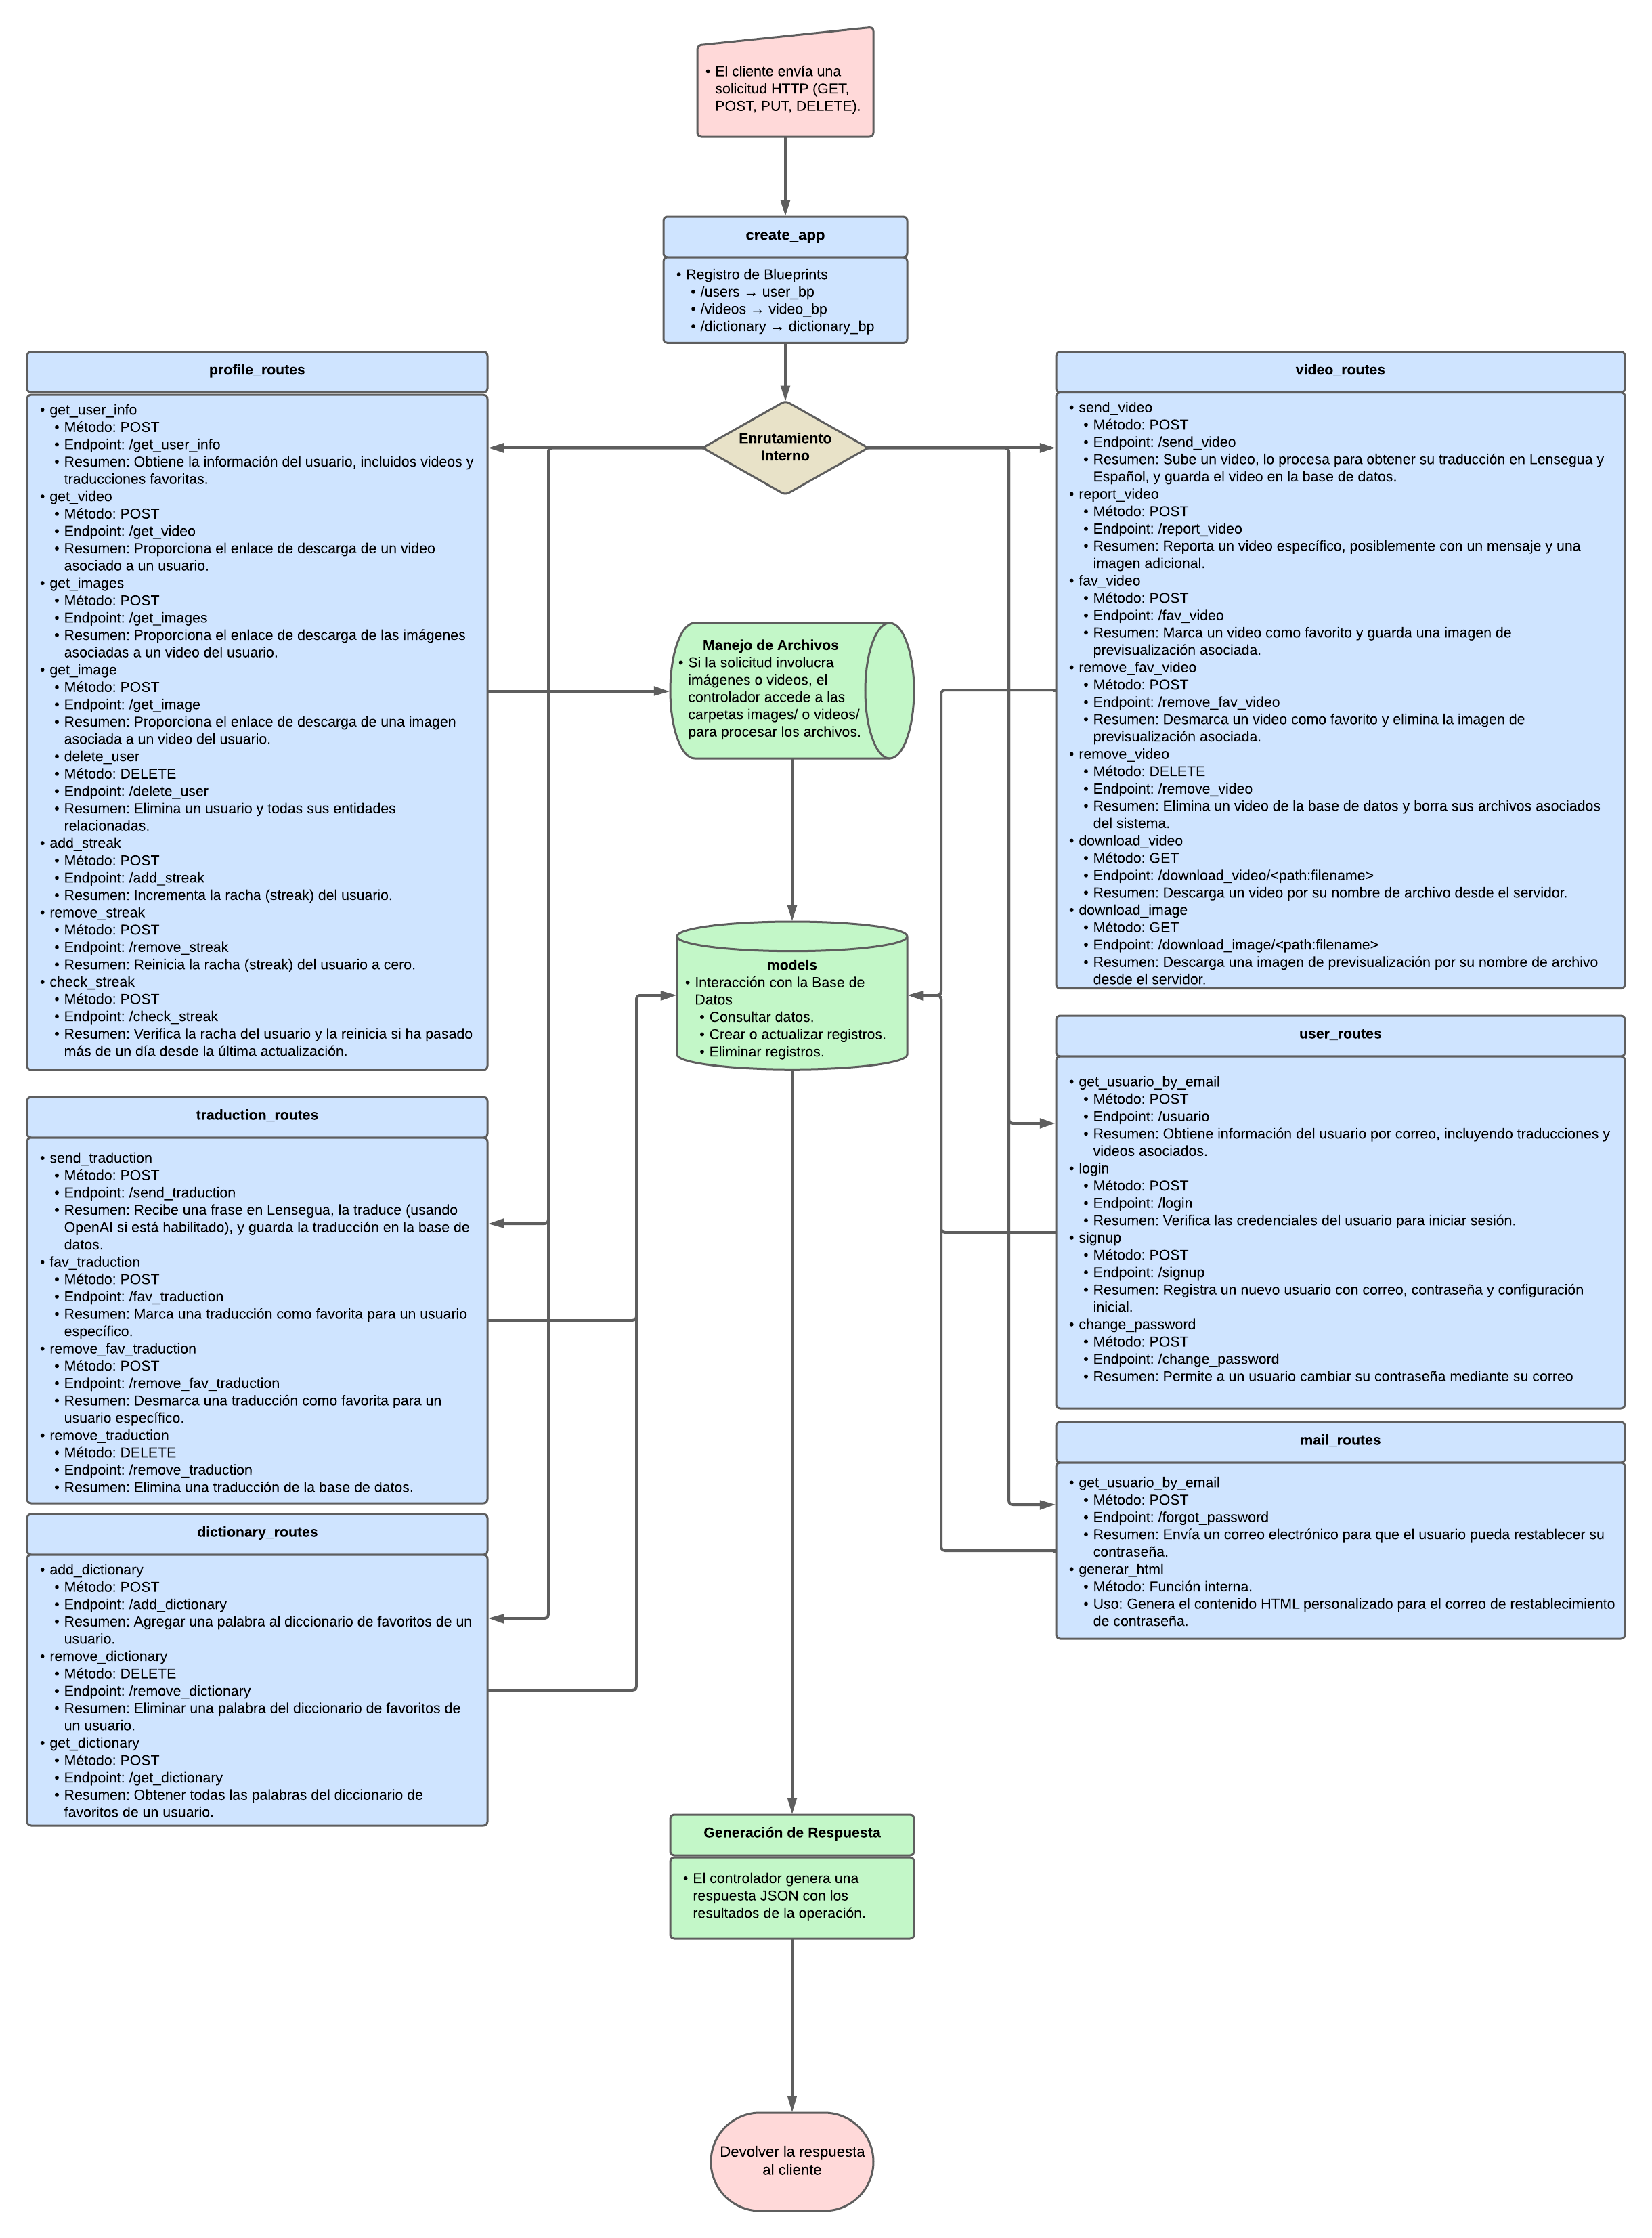
\includegraphics[width=0.5\textwidth]{figuras/diagrama_flujo.png}
    \caption{Diagrama de flujo.}
    \label{fig:diagrama_flujo}
\end{figure}

%Aqui vamos a meter lo del status y como el hacer el inicio del sistema de api-central que pues aqui se resume bien chilero y meter imagen de api-centralServiceStatus

\subsection{Implementación de Flask con GUnicorn y NGinx}

% Configuración para resaltar el código de Nginx
\lstset{
    basicstyle=\ttfamily,
    keywordstyle=\color{blue},
    frame=single,
    numbers=left,
    numberstyle=\tiny,
    breaklines=true,
    backgroundcolor=\color{gray!10}
}

% img: DiagramaImplementacionGU-NG.png
\subsection*{Componentes Principales}

\begin{enumerate}[label=\alph*)]
    \item \textbf{Flask}: Framework de Python utilizado para construir la lógica de la aplicación.
    \item \textbf{Gunicorn}: Servidor WSGI que ejecuta la aplicación Flask en un entorno de producción.
    \item \textbf{Nginx}: Proxy inverso que maneja las solicitudes del cliente, distribuye la carga, y mejora la seguridad.
\end{enumerate}

\subsection*{Flujo de trabajo del sistema de APIs:}

\begin{figure}[H]
    \centering
    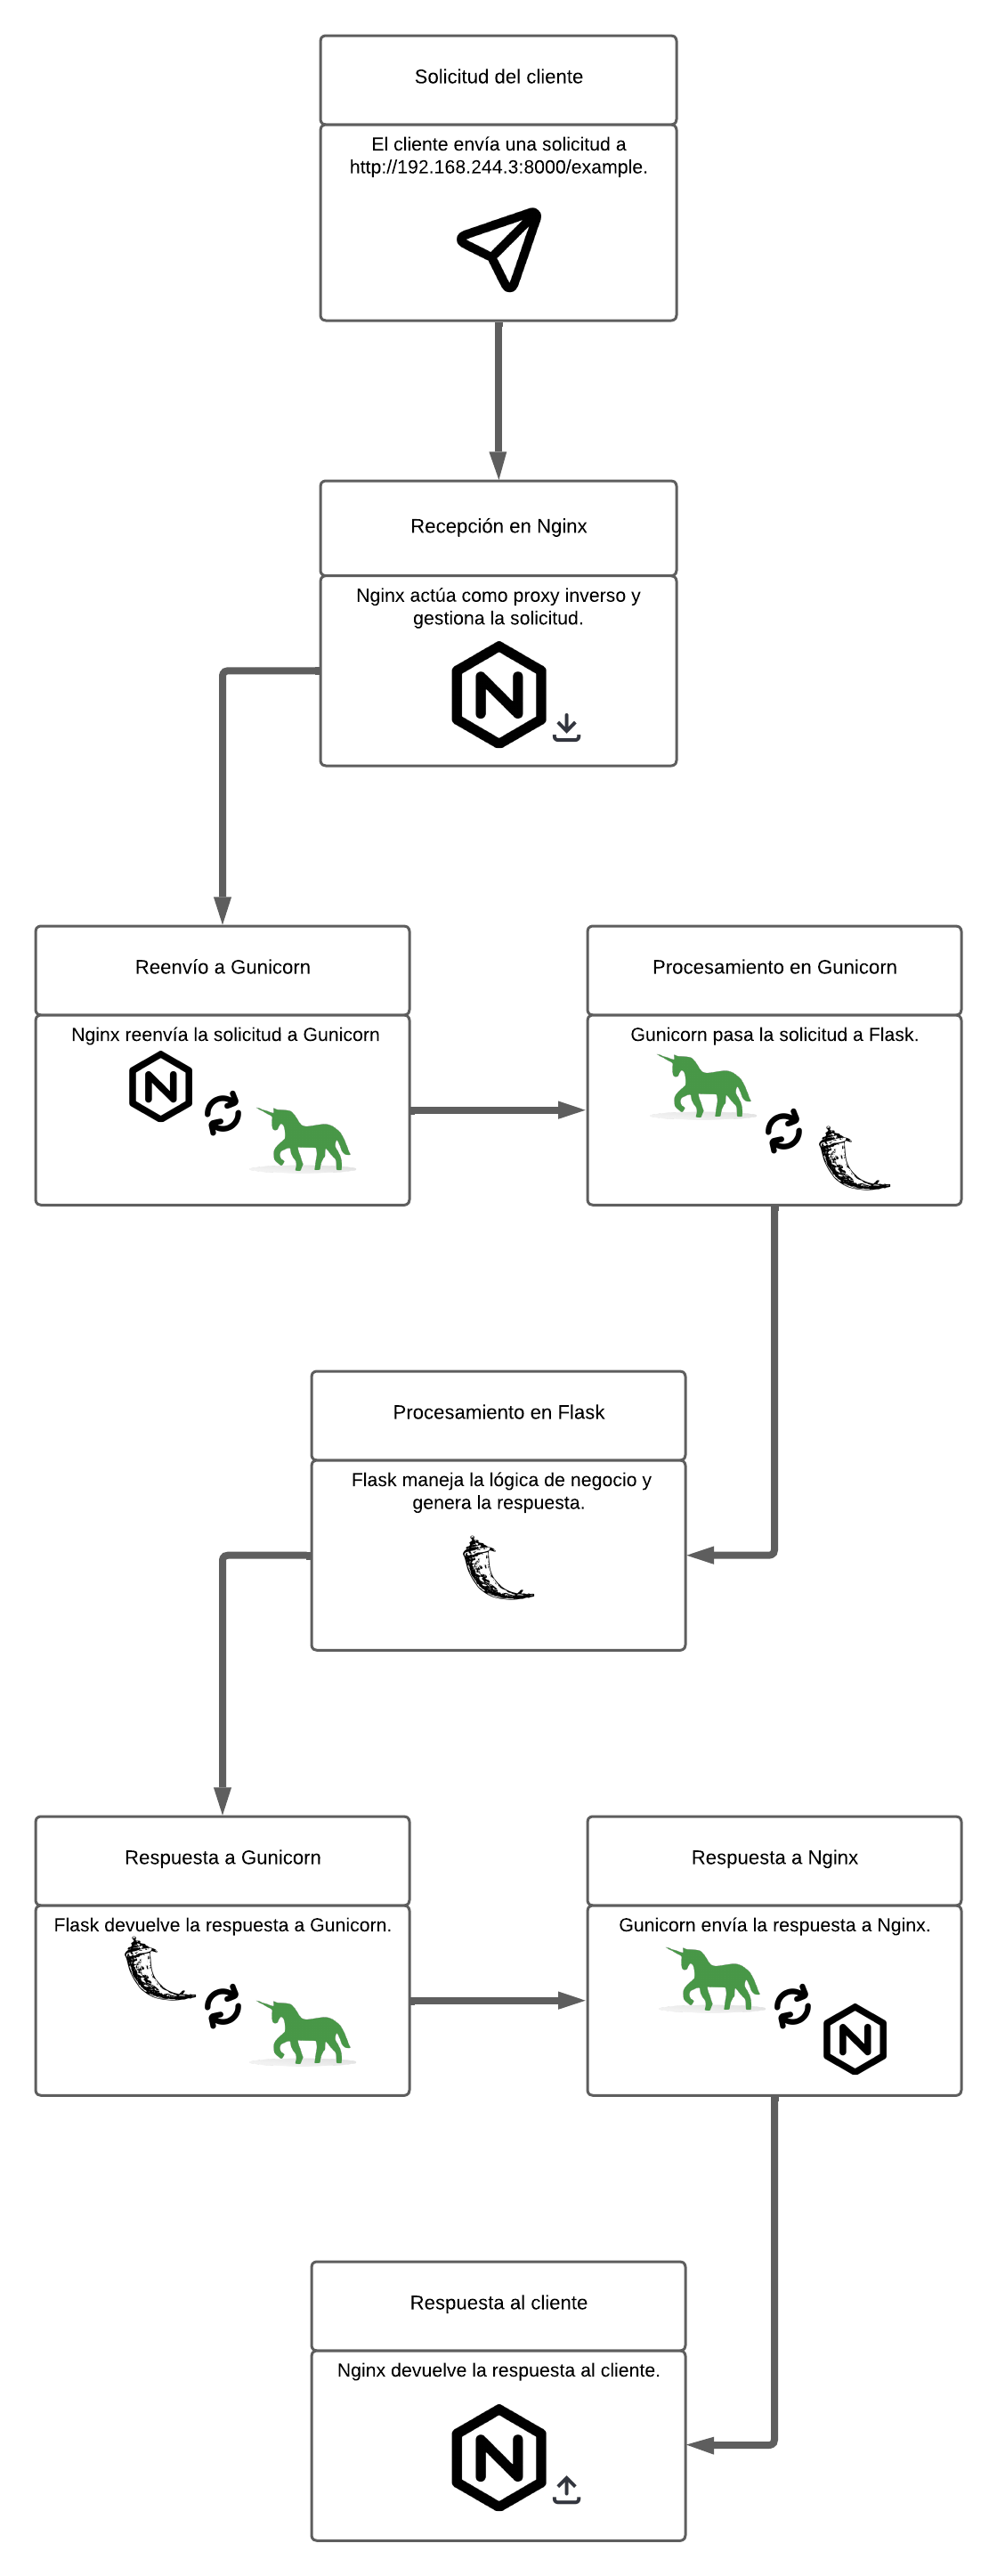
\includegraphics[width=0.5\textwidth]{figuras/DiagramaImplementacionGU-NG.png}
    \caption{Flujo de trabajo completo del sistema de APIs.}
    \label{fig:DiagramaImplementacionGU-NG}
\end{figure}

\section*{Configuración general}

\subsection*{a. Configuración de Flask}
La aplicación Flask fue configurada con soporte para migraciones de bases de datos, utilizando SQLAlchemy y Flask-Migrate. Esta configuración permite la manipulación sencilla de esquemas de bases de datos a medida que se añaden nuevas funcionalidades al sistema.

\subsection*{b. Configuración de Gunicorn}
\begin{enumerate}[label=\roman*.]
    \item Gunicorn se seleccionó como el servidor WSGI debido a su capacidad para manejar múltiples solicitudes concurrentes mediante el uso de workers. Gunicorn se ejecuta vinculándose a todas las interfaces de red en un puerto específico, lo que permite que la aplicación esté disponible en la red local o en internet.
    \item Para gestionar múltiples procesos de Gunicorn, se configuró su ejecución como un servicio del sistema. Esto asegura que Gunicorn inicie automáticamente con el sistema y facilite la gestión del servidor en producción.
\end{enumerate}

\subsection*{c. Configuración de Nginx}
\begin{enumerate}[label=\roman*.]
    \item Nginx se configuró como un proxy inverso para manejar la entrada de solicitudes del cliente y distribuirlas a Gunicorn. Este paso es crucial para manejar eficientemente la concurrencia y asegurar que el tráfico de red no sobrecargue el servidor de aplicaciones.
\end{enumerate}

\subsection*{d. Archivo de configuración de Nginx:}

\begin{lstlisting}[language=bash, caption={Archivo de configuración de Nginx.}]
server {
    listen 4242;
    server_name 192.168.244.3;

    location / {
        proxy_pass http://unix:/srv/web-apps/api-central/api-central.sock;
        include proxy_params;
        proxy_redirect off;
    }
}
\end{lstlisting}

\subsection*{Explicación del archivo de configuración de Nginx:}

\begin{enumerate}[label=\roman*.]
    \item \textbf{listen 4242}: Especifica el puerto en el que Nginx escuchará las solicitudes.
    \item \textbf{server\_name 192.168.244.3}: Define la dirección IP del servidor.
    \item \textbf{proxy\_pass}: Redirige las solicitudes recibidas a Gunicorn mediante un socket Unix, lo que mejora el rendimiento y la seguridad al evitar conexiones TCP adicionales.
    \item \textbf{include proxy\_params}: Incluye parámetros comunes para proxies inversos en Nginx.
    \item \textbf{proxy\_redirect off}: Desactiva la redirección automática de respuestas, permitiendo un control más preciso sobre el flujo de la solicitud y respuesta.
\end{enumerate}

\subsection{Implementación de SQLAlchemy para manejo de base de datos y entidades}

% AQUI: colocar imagen de migracionSqlAlchemy

\subsubsection*{1. Definición de Entidades}
Las entidades en SQLAlchemy se definen como clases que heredan de \texttt{db.Model}. Cada clase representa una tabla en la base de datos, y sus atributos corresponden a las columnas de la tabla. Por ejemplo, una entidad \texttt{Usuario} se define para representar la tabla \texttt{usuarios} con columnas como \texttt{id}, \texttt{correo} y \texttt{contrasena}. Estas clases se definen en un archivo específico, como \texttt{models.py}, para mantener el código organizado y escalable.

\subsubsection*{2. Relación entre Entidades}
SQLAlchemy permite definir relaciones entre entidades usando claves foráneas (\textit{ForeignKey}). Por ejemplo, en la entidad \texttt{Video}, existe una relación con la entidad \texttt{Usuario} mediante la columna \texttt{usuario\_id}, que referencia al \texttt{id} de la tabla \texttt{usuarios}. Este tipo de relaciones permiten manejar estructuras de datos más complejas y realizar consultas entre tablas relacionadas de forma sencilla.

\subsubsection*{3. Migraciones de Base de Datos}
Flask-Migrate se utiliza para aplicar cambios en el esquema de la base de datos de manera controlada. Una vez que las entidades están definidas, Flask-Migrate permite generar y aplicar migraciones para reflejar estos modelos en la base de datos. Este proceso se realiza en tres pasos:

\begin{enumerate}[label=\alph*.]
    \item \textbf{Inicialización de las Migraciones}: Se configura Flask-Migrate para gestionar la base de datos.
    \item \textbf{Creación de Migraciones}: Cada vez que se añade o modifica una entidad, se genera una nueva migración.
    \item \textbf{Aplicación de Migraciones}: Las migraciones se aplican a la base de datos, creando o modificando las tablas según sea necesario.
\end{enumerate}

\subsubsection*{4. Operaciones CRUD}
Con SQLAlchemy, las operaciones CRUD (Crear, Leer, Actualizar, Eliminar) se manejan fácilmente mediante el uso de sesiones de base de datos. Estas sesiones permiten realizar consultas, insertar nuevos registros, actualizar datos existentes y eliminar registros, todo de una manera declarativa y fluida.

\subsection{Implementación de módulo API para bases de datos}

Para facilitar las consultas y las inserciones de datos, se utilizará Flask como framework principal debido a su ligereza y capacidad para manejar peticiones de manera eficiente. Este módulo API permitirá un manejo flexible de diferentes formatos de datos, incluyendo videos y texto. La estructura del módulo está diseñada para optimizar el rendimiento del sistema, minimizando el uso de recursos y maximizando la velocidad de respuesta, lo que es crucial para procesar y responder a las interacciones de los usuarios en tiempo real.

% Detalle de las APIs en formato de lista
\textbf{Módulo: Procesamiento de lenguaje}
\begin{itemize}
    \item \textbf{Nombre de la API}: \texttt{API\_Procesamiento\_de\_Lenguaje}
    \item \textbf{Función de la API}: Procesar texto y generar respuestas basadas en el modelo
    \item \textbf{Entrada}: XML con texto
    \item \textbf{Salida Esperada}: Respuesta en XML del modelo GPT-4
\end{itemize}

\textbf{Módulo: Llama}
\begin{itemize}
    \item \textbf{Nombre de la API}: \texttt{API\_Llama}
    \item \textbf{Función de la API}: Analizar y responder consultas con el modelo Llama
    \item \textbf{Entrada}: XML con consulta
    \item \textbf{Salida Esperada}: Respuesta en XML del modelo Llama
\end{itemize}

\textbf{Módulo: Visión por computadora}
\begin{itemize}
    \item \textbf{Nombre de la API}: \texttt{API\_Vision}
    \item \textbf{Función de la API}: Analizar imágenes y videos, y detectar objetos
    \item \textbf{Entrada}: XML con imagen/video
    \item \textbf{Salida Esperada}: Respuesta en XML con análisis de visión por computadora
\end{itemize}

\textbf{Módulo: HyperVisor}
\begin{itemize}
    \item \textbf{Nombre de la API}: \texttt{API\_HyperVisor}
    \item \textbf{Función de la API}: Gestionar y monitorizar las máquinas virtuales
    \item \textbf{Entrada}: XML con comandos
    \item \textbf{Salida Esperada}: Respuesta en XML con estado de VMs
\end{itemize}

\subsection{API para integración de modelos de procesamiento}

Se desarrollará una API específica para facilitar la interacción entre el módulo de visión por computadora y los modelos de lenguaje natural. Esta API asegurará que la información fluya de manera eficiente desde la recepción de videos hasta la entrega de resultados en texto o voz, pasando por la consulta de bases de datos. La arquitectura de red y del servidor será diseñada para manejar altas demandas de solicitudes sin degradar la calidad del servicio, utilizando técnicas de balanceo de carga y optimización de recursos para garantizar un proceso robusto y confiable.

Se diseñará un entorno virtualizado utilizando Multipass sobre un servidor con Ubuntu 22.08 ya instalado, lo que facilitará la segregación de los módulos de visión por computadora, inteligencia artificial con GPT-4 y el modelo de IA Llama. Cada uno de estos módulos operará dentro de su propia máquina virtual, configurada específicamente para satisfacer sus requisitos operativos y de procesamiento.

Para iniciar el proceso, se configurarán máquinas virtuales individuales para cada módulo bajo el hypervisor Multipass en Ubuntu 22.08. Esta configuración implica la asignación de los recursos necesarios, como CPU dedicada, memoria RAM adecuada y espacio de almacenamiento suficiente, de acuerdo con las demandas específicas de cada aplicación. Además, se establecerán redes virtuales que permitan una comunicación eficaz y segura entre las máquinas virtuales y los sistemas de bases de datos externos.

\subsection{Implementación de Crontab}

Para garantizar que los usuarios mantengan una racha activa y que se reinicie automáticamente si ha pasado más de un día sin actividad, se ha implementado un proceso automatizado utilizando `crontab` en el servidor Linux. Esta tarea se ejecuta todos los días a las 3:00 a.m. y ejecuta un script de Python que revisa la última hora de actualización de la racha de cada usuario y la reinicia si ha pasado más de 24 horas desde la última actualización.

\subsubsection{Configuración del Cron Job}

Para configurar la tarea programada que se ejecuta a las 3:00 a.m. todos los días, se debe agregar la siguiente línea al archivo de crontab del usuario adecuado:

\lstset{
    basicstyle=\ttfamily\small,
    numbers=left,
    numberstyle=\tiny\color{gray},
    backgroundcolor=\color{lightgray!20},
    frame=single,
    captionpos=b,
    breaklines=true,
    tabsize=4,
    showstringspaces=false
}

\begin{lstlisting}[caption={Frecuencia de ejecución}, label={lst:cron_frequency}]
0 3 * * *
\end{lstlisting}
\noindent
Indica la frecuencia de ejecución (todos los días a las 3:00 a.m.).

\begin{lstlisting}[caption={Ruta al intérprete de Python}, label={lst:python_path}]
/usr/bin/python3
\end{lstlisting}
\noindent
Es la ruta al intérprete de Python.

\begin{lstlisting}[caption={Ruta al script de Python}, label={lst:script_path}]
/ruta/al/script/reset_streaks.py
\end{lstlisting}
\noindent
Es la ruta completa al script de Python que contiene la lógica de reinicio de rachas.

\begin{lstlisting}[caption={Redirección de salida y errores}, label={lst:log_redirection}]
>> /ruta/al/log/reset_streaks.log 2>&1
\end{lstlisting}
\noindent
Redirige la salida y los errores del script a un archivo de log para facilitar la revisión de su ejecución.

El script de Python que se ejecuta está diseñado para realizar las siguientes tareas:
\begin{enumerate}
    \item Crear una aplicación Flask y un contexto de aplicación para que el script pueda interactuar con la base de datos.
    \item Obtener todos los usuarios de la base de datos y revisar su última hora de actualización de racha.
    \item Calcular la diferencia de tiempo entre la hora actual y la última actualización. Si ha pasado más de 24 horas, reiniciar la racha del usuario y actualizar la hora de la última modificación.
    \item Registrar la acción en la base de datos y mostrar un mensaje de confirmación en la consola.
\end{enumerate}

\noindent
El código del script es el siguiente:

\lstset{
    language=Python,
    basicstyle=\ttfamily\small,
    numbers=left,
    numberstyle=\tiny\color{gray},
    backgroundcolor=\color{lightgray!20},
    frame=single,
    captionpos=b,
    breaklines=true,
    tabsize=4,
    showstringspaces=false
}

\begin{lstlisting}[caption={Script de restablecimiento de streaks en Flask}, label={lst:reset_streaks}]
from app import create_app, db
from app.models import User
from datetime import datetime, timedelta

# Crear la aplicación Flask y contexto
app = create_app()
app.app_context().push()

def reset_streaks():
    # Obtener todos los usuarios
    users = User.query.all()
    for usuario in users:
        if usuario.last_streak_update:
            # Calcular la diferencia de tiempo desde la última actualización
            delta = datetime.utcnow() - usuario.last_streak_update
            if delta > timedelta(days=1):
                # Ha pasado más de un día, reiniciar el streak
                usuario.streak = 0
                usuario.last_streak_update = datetime.utcnow()
                db.session.commit()
                print(f"Streak reset for user {usuario.mail}")

if __name__ == "__main__":
    reset_streaks()
\end{lstlisting}

\subsubsection{Importancia de la Implementación}

El uso de `crontab` para esta tarea es fundamental para mantener la consistencia y la precisión en el control de rachas de los usuarios sin intervención manual. Esto garantiza que las rachas de los usuarios se gestionen de manera automatizada, promoviendo un comportamiento constante y ofreciendo una mejor experiencia de usuario. Además, el uso de `crontab` permite que la tarea se ejecute en horarios de baja actividad del servidor, minimizando el impacto en el rendimiento del sistema.


\section{Virtualización del servidor para múltiples modelos}

\section*{Implementación de arquitectura con máquinas virtuales}

Para implementar esta arquitectura, se crearán un total de tres máquinas virtuales adicionales al servidor principal que actuará como HOST. Cada máquina virtual será dedicada a uno de los módulos: visión por computadora, inteligencia artificial con GPT-4 y el modelo de IA Llama.

Utilizando Multipass sobre Ubuntu 22.08, cada máquina virtual se configurará meticulosamente para cumplir con los requisitos específicos de procesamiento, asignando CPU dedicadas, memoria RAM adecuada y espacio de almacenamiento suficiente. Además, se establecerán redes virtuales para asegurar una comunicación eficiente y segura entre las máquinas virtuales y los sistemas de bases de datos. Esta configuración garantizará que cada módulo opere de manera independiente y óptima, permitiendo un procesamiento robusto y confiable bajo altas demandas de solicitudes sin comprometer la calidad del servicio.

\subsection*{Resumen del Sistema:}

\renewcommand{\arraystretch}{1.3} % Aumenta la altura de las filas
\begin{table}[H]
\centering
\begin{tabularx}{\textwidth}{|m{4cm}|m{6cm}|m{4cm}|}
\hline
\textbf{Memoria RAM} & \textbf{Espacio en disco} & \textbf{CPU} \\ \hline
Total: 125 GiB & /dev/mapper/ubuntu--vg-ubuntu--lv: 98G total, 19G usado, 75G disponible (20\% uso) & Arquitectura: x86\_64 \\ \hline
Usada: 50 MiB & /dev/sda2: 2.0G total, 253M usado, 1.6G disponible (14\% uso) & CPUs: 32 (Intel(R) Xeon(R) Silver 4216 CPU @ 2.10GHz) \\ \hline
Libre: 75 GiB & /dev/sda1: 1.1G total, 6.1M usado, 1.1G disponible (1\% uso) & Núcleos por CPU: 16 \\ \hline
Disponible: 123 GiB & & Hilos por núcleo: 2 \\ \hline
Swap Total: 8.0 GiB & & Virtualización: VT-x \\ \hline
Swap Usada: 0B & & \\ \hline
\end{tabularx}
\caption{Resumen del sistema}
\label{tab:system_summary}
\end{table}

El uso de técnicas de balanceo de carga y la optimización de recursos serán esenciales para garantizar que el sistema pueda manejar altos volúmenes de solicitudes sin comprometer la calidad del servicio. Cada máquina virtual se configurará con las dependencias y bibliotecas necesarias, garantizando que los módulos de visión por computadora y los modelos de IA operen de manera óptima y confiable dentro de este entorno virtualizado controlado.

Parte de este balanceo implica la distribución de recursos entre las máquinas virtuales. Para esto, se dividieron los recursos entre las máquinas de la siguiente manera:

\renewcommand{\arraystretch}{1.3} % Aumenta la altura de las filas
\begin{table}[H]
\centering
\begin{tabularx}{\textwidth}{|m{4.5cm}|m{4cm}|X|}
\hline
\textbf{Máquina Virtual 1 (VM1)} & \textbf{RAM: 32 GiB} & \textbf{CPUs: 8} \\ \hline
\textbf{Máquina Virtual 2 (VM2)} & \textbf{RAM: 32 GiB} & \textbf{CPUs: 8} \\ \hline
\textbf{Máquina Virtual 3 (VM3)} & \textbf{RAM: 32 GiB} & \textbf{CPUs: 8} \\ \hline
\textbf{Host (host de VM)} & \textbf{RAM: 30 GiB (restante)} & \textbf{CPUs: 8 (restante)} \\ \hline
\end{tabularx}
\caption{Distribución de recursos entre las máquinas virtuales y el host}
\label{tab:vm_resources}
\end{table}

\vspace{0.5cm}

\begin{figure}[H]
    \centering
    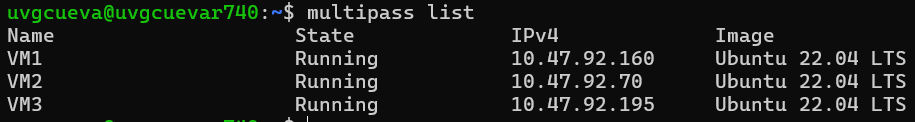
\includegraphics[width=0.5\textwidth]{figuras/EstadosVMs.png}
    \caption{Estado de las máquinas virtuales dentro del sistema}
    \label{fig:EstadosVMs}
\end{figure}

\section{Implementación de pruebas de eficiencia}

\begin{enumerate}
    \item \textbf{Instalación de Herramientas de Monitoreo:}
    \begin{enumerate}[label*=\alph*.]
        \item Instalar el agente NGINX Amplify para monitorear el uso de recursos (CPU, memoria, disco y red) en tiempo real.
        \item Adicionalmente, instalar herramientas complementarias como \texttt{htop}, \texttt{dstat}, \texttt{iotop}, \texttt{nload} y \texttt{sysdig} para monitoreo detallado y comparación de métricas.
    \end{enumerate}

    \item \textbf{Preparación del Entorno de Pruebas:}
    \begin{enumerate}[label*=\alph*.]
        \item Desarrollar un script en Python que realice solicitudes a las APIs, utilizando librerías como \texttt{requests} para solicitudes HTTP y \texttt{psutil} para monitoreo de recursos.
        \item Configurar el sistema de logging para registrar métricas en un archivo de log y enviar datos al agente NGINX Amplify.
    \end{enumerate}

    \item \textbf{Monitoreo Continuo:}
    \begin{enumerate}[label*=\alph*.]
        \item Monitorizar los recursos del sistema en tiempo real utilizando NGINX Amplify y las herramientas complementarias instaladas.
        \item Registrar métricas clave como el uso de CPU, memoria, disco y red durante las pruebas.
        \item Configurar alertas en NGINX Amplify para notificaciones automáticas sobre uso excesivo de recursos.
    \end{enumerate}

    \item \textbf{Análisis de Resultados:}
    \begin{enumerate}[label*=\alph*.]
        \item Revisar los logs generados durante las pruebas para evaluar el tiempo de respuesta y la utilización de recursos.
        \item Utilizar el panel de NGINX Amplify para analizar métricas históricas y tendencias de rendimiento.
        \item Identificar cuellos de botella y áreas de mejora mediante las métricas y gráficos proporcionados por NGINX Amplify.
    \end{enumerate}

    \item \textbf{Optimización y Repetición de Pruebas:}
    \begin{enumerate}[label*=\alph*.]
        \item Implementar ajustes necesarios en la configuración del servidor y las aplicaciones basados en los resultados del análisis.
        \item Repetir las pruebas para verificar las mejoras en el rendimiento del sistema.
        \item Continuar el ciclo de pruebas y optimización hasta alcanzar un rendimiento óptimo, utilizando NGINX Amplify para validar las mejoras.
    \end{enumerate}
\end{enumerate}

\section{Pruebas de Carga}

\subsection{Objetivo}
El objetivo de las pruebas de carga es evaluar el rendimiento del sistema bajo condiciones de carga esperadas, simulando múltiples usuarios y solicitudes concurrentes para determinar la capacidad del sistema. Estas pruebas permiten identificar posibles áreas de mejora en la infraestructura y el manejo de recursos.

\subsection{Procedimiento}
\begin{enumerate}
    \item \textbf{Simulación de Usuarios}: Se desarrolló un script en Python para crear múltiples usuarios simulados. La función \texttt{create\_users} crea registros y datos de autenticación de usuario, almacenándolos para reutilización durante la prueba.
    \item \textbf{Acciones Concurrentes}: Una vez autenticados, cada usuario simulado ejecuta una serie de acciones concurrentes usando \texttt{ThreadPoolExecutor}:
    \begin{itemize}
        \item Obtiene su información de perfil (\texttt{get\_user\_info}).
        \item Incrementa su racha de actividad (\texttt{add\_streak}).
        \item Realiza operaciones de video y traducción (subida de video, recuperación, marcación como favorito).
    \end{itemize}
    \item \textbf{Medición de Tiempos de Respuesta}: La función \texttt{send\_request} mide el tiempo de respuesta de cada operación y el estado HTTP. Esto permite registrar tiempos de respuesta y determinar si el sistema mantiene la estabilidad bajo carga.
\end{enumerate}

Para evaluar la capacidad de nuestro servidor y entender sus límites de rendimiento, realizamos una serie de pruebas de carga incrementales. Estas pruebas consistieron en simular un número creciente de usuarios concurrentes interactuando con el sistema, comenzando con 50 usuarios y aumentando progresivamente hasta 1100 usuarios. El objetivo de este enfoque es aplicar niveles crecientes de estrés en el servidor, analizando cómo responde bajo diferentes cargas de trabajo.

Cada prueba de carga permite observar el tiempo de respuesta y la estabilidad del sistema a medida que la cantidad de usuarios aumenta, identificando el punto en el que el rendimiento empieza a degradarse significativamente. Esta metodología nos ayuda a determinar la capacidad máxima de usuarios concurrentes que nuestro servidor puede manejar de forma estable antes de experimentar problemas críticos, como demoras excesivas o fallos en el procesamiento de las solicitudes. Además, este proceso de pruebas graduales nos permite identificar las métricas críticas que influencian el desempeño, tales como la utilización de CPU, la memoria disponible y el tiempo de respuesta de las solicitudes.

\newpage

%tenemos que cargar las imagenes pruebaCarga50U.png
%tenemos que cargar las imagenes pruebaCarga100U.png
%tenemos que cargar las imagenes pruebaCarga200U.png
%tenemos que cargar las imagenes pruebaCarga300U.png
%tenemos que cargar las imagenes pruebaCarga400U.png
%tenemos que cargar las imagenes pruebaCarga500U.png
%tenemos que cargar las imagenes pruebaCarga600U.png
%tenemos que cargar las imagenes pruebaCarga700U.png
%tenemos que cargar las imagenes pruebaCarga800U.png
%tenemos que cargar las imagenes pruebaCarga900U.png
%tenemos que cargar las imagenes pruebaCarga1100U.png
\begin{figure}[H]
    \centering
    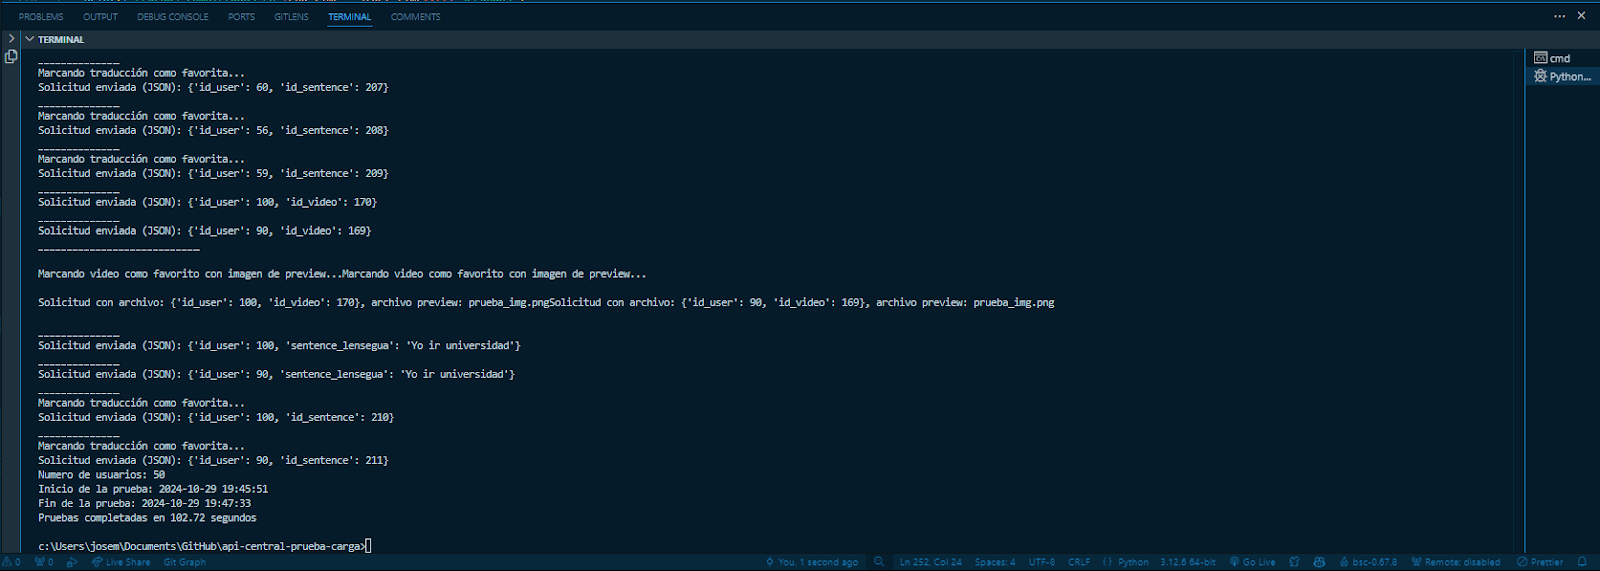
\includegraphics[width=0.5\textwidth]{figuras/pruebaCarga50U.png}
    \caption{Resultados de la prueba de carga con 50 usuarios concurrentes.}
    \label{fig:pruebaCarga50U}
\end{figure}

\begin{figure}[H]
    \centering
    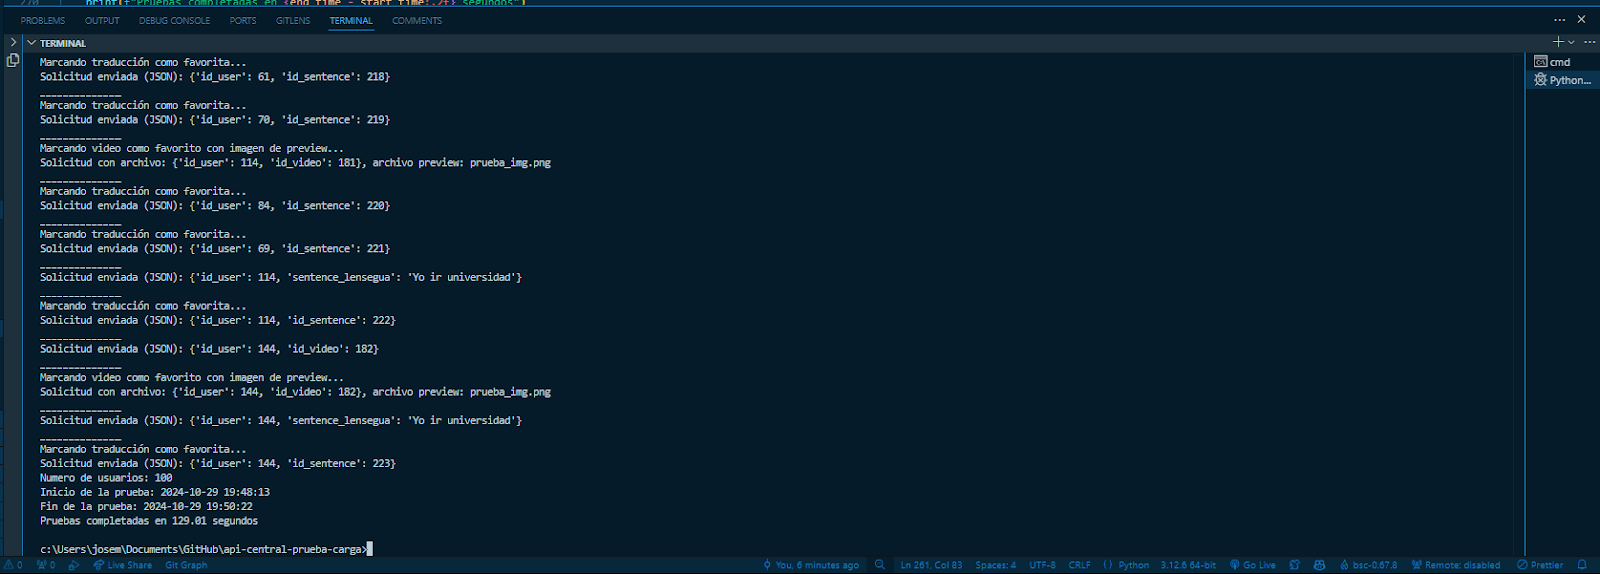
\includegraphics[width=0.5\textwidth]{figuras/pruebaCarga100U.png}
    \caption{Resultados de la prueba de carga con 100 usuarios concurrentes.}
    \label{fig:pruebaCarga100U}
\end{figure}

\begin{figure}[H]
    \centering
    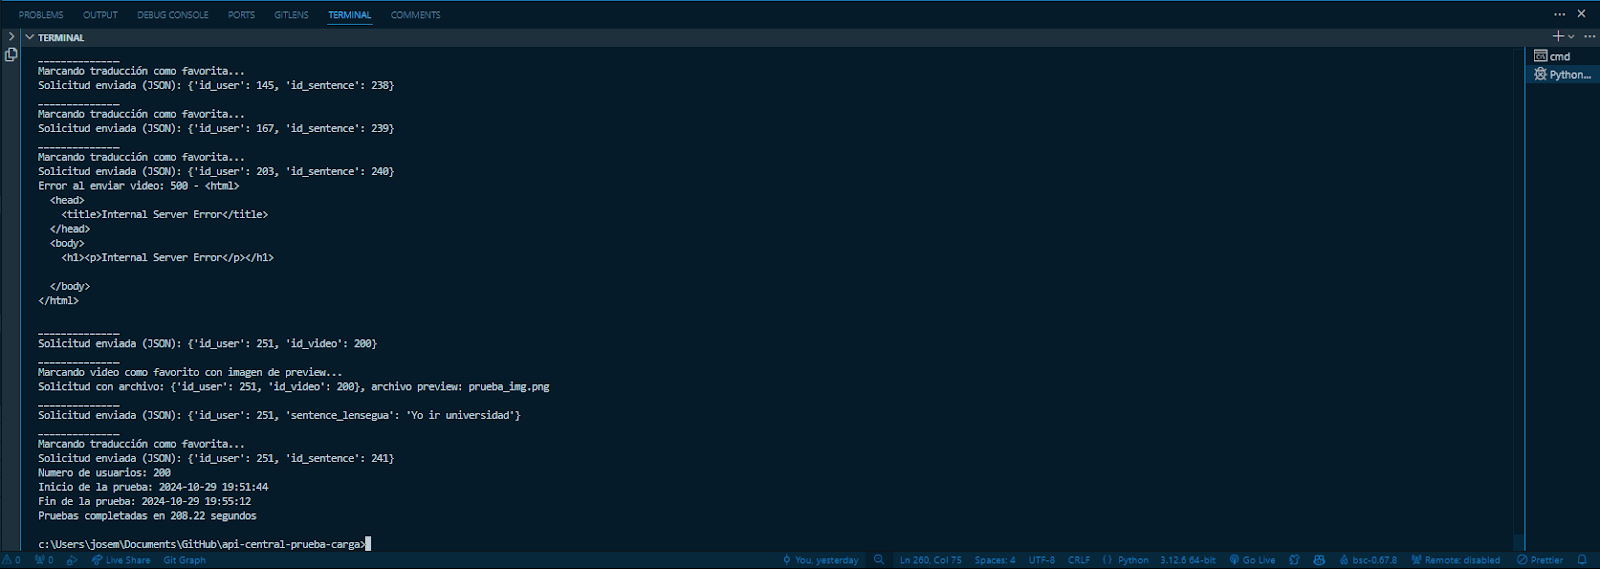
\includegraphics[width=0.5\textwidth]{figuras/pruebaCarga200U.png}
    \caption{Resultados de la prueba de carga con 200 usuarios concurrentes.}
    \label{fig:pruebaCarga200U}
\end{figure}

\begin{figure}[H]
    \centering
    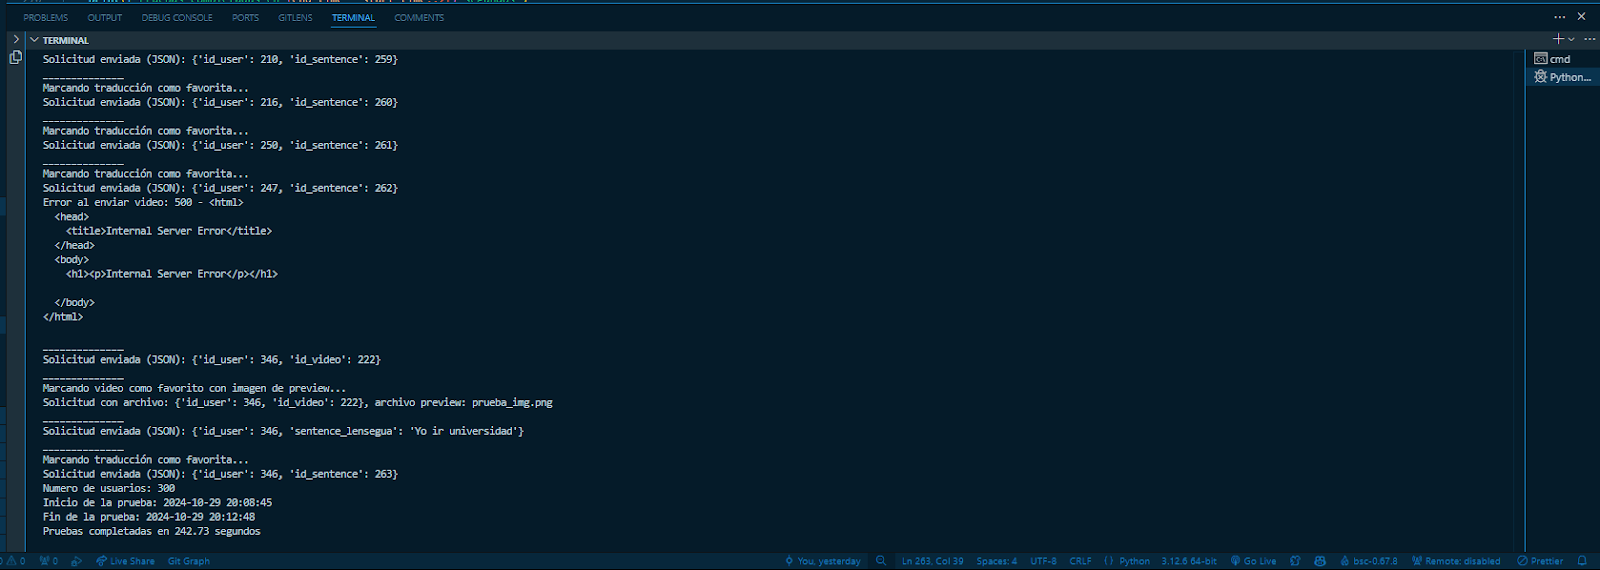
\includegraphics[width=0.5\textwidth]{figuras/pruebaCarga300U.png}
    \caption{Resultados de la prueba de carga con 300 usuarios concurrentes.}
    \label{fig:pruebaCarga300U}
\end{figure}

\begin{figure}[H]
    \centering
    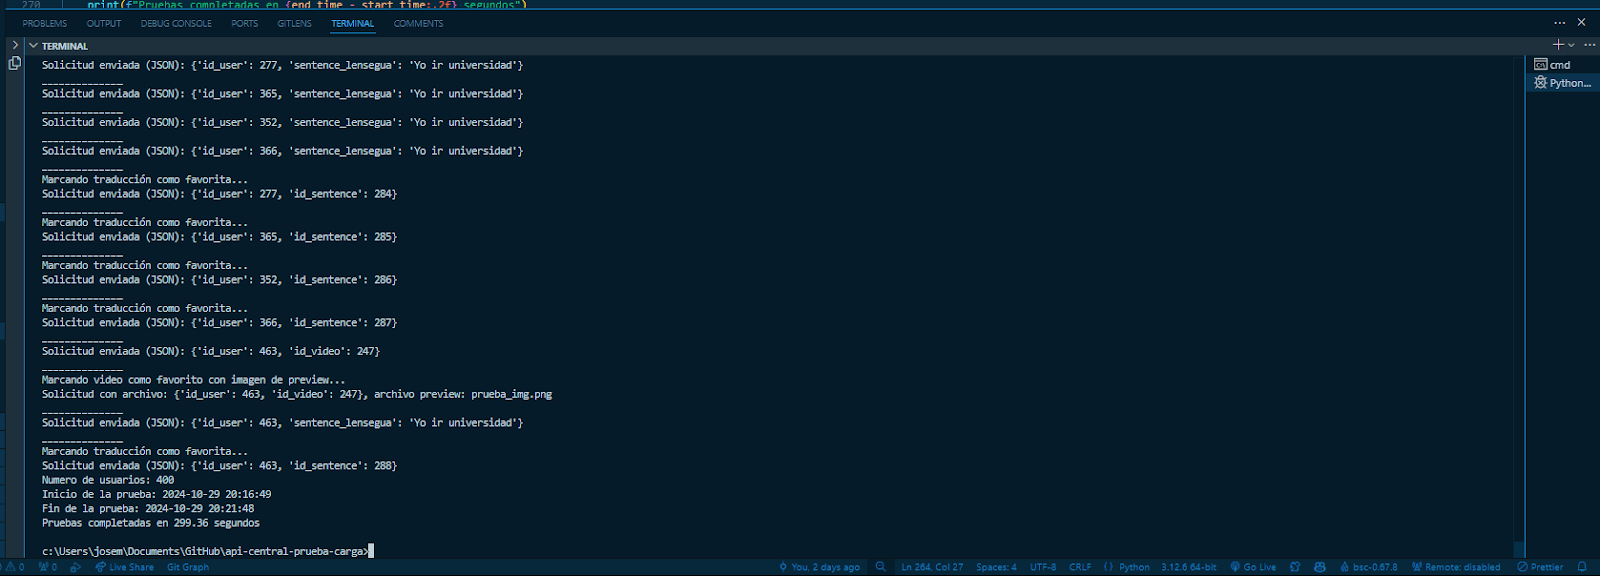
\includegraphics[width=0.5\textwidth]{figuras/pruebaCarga400U.png}
    \caption{Resultados de la prueba de carga con 400 usuarios concurrentes.}
    \label{fig:pruebaCarga400U}
\end{figure}

\begin{figure}[H]
    \centering
    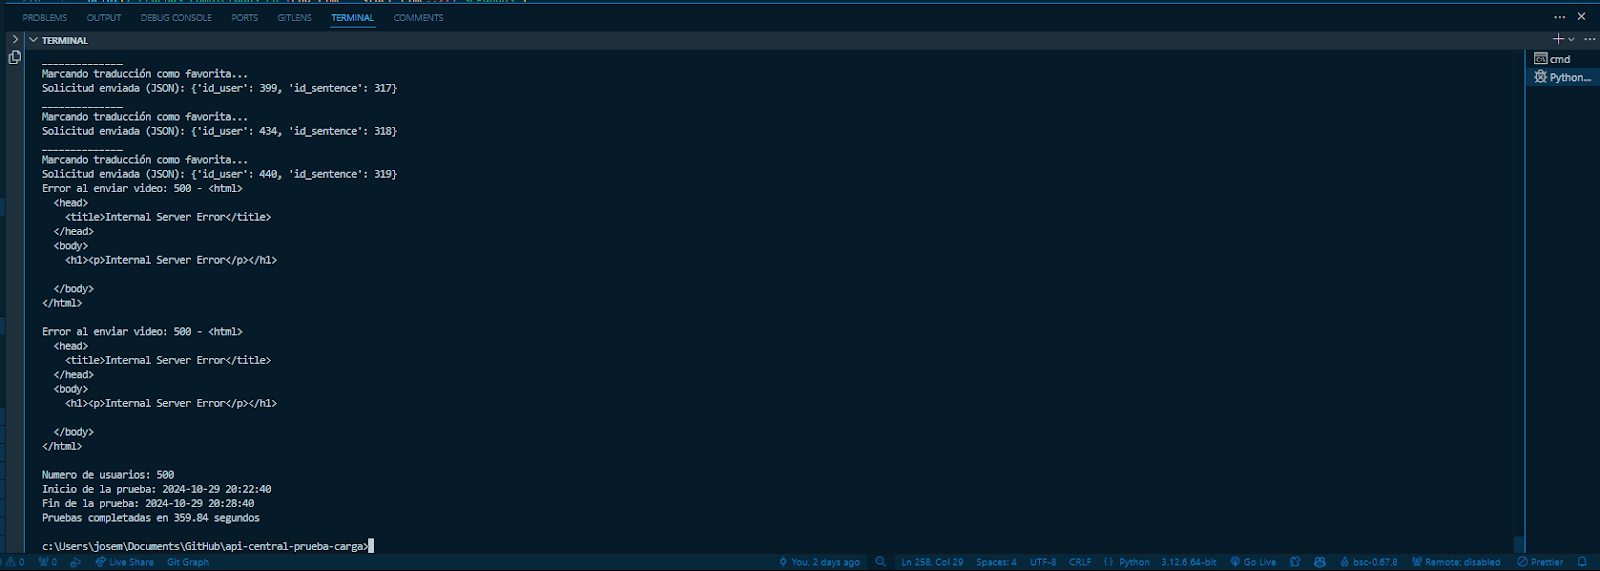
\includegraphics[width=0.5\textwidth]{figuras/pruebaCarga500U.png}
    \caption{Resultados de la prueba de carga con 500 usuarios concurrentes.}
    \label{fig:pruebaCarga500U}
\end{figure}

\begin{figure}[H]
    \centering
    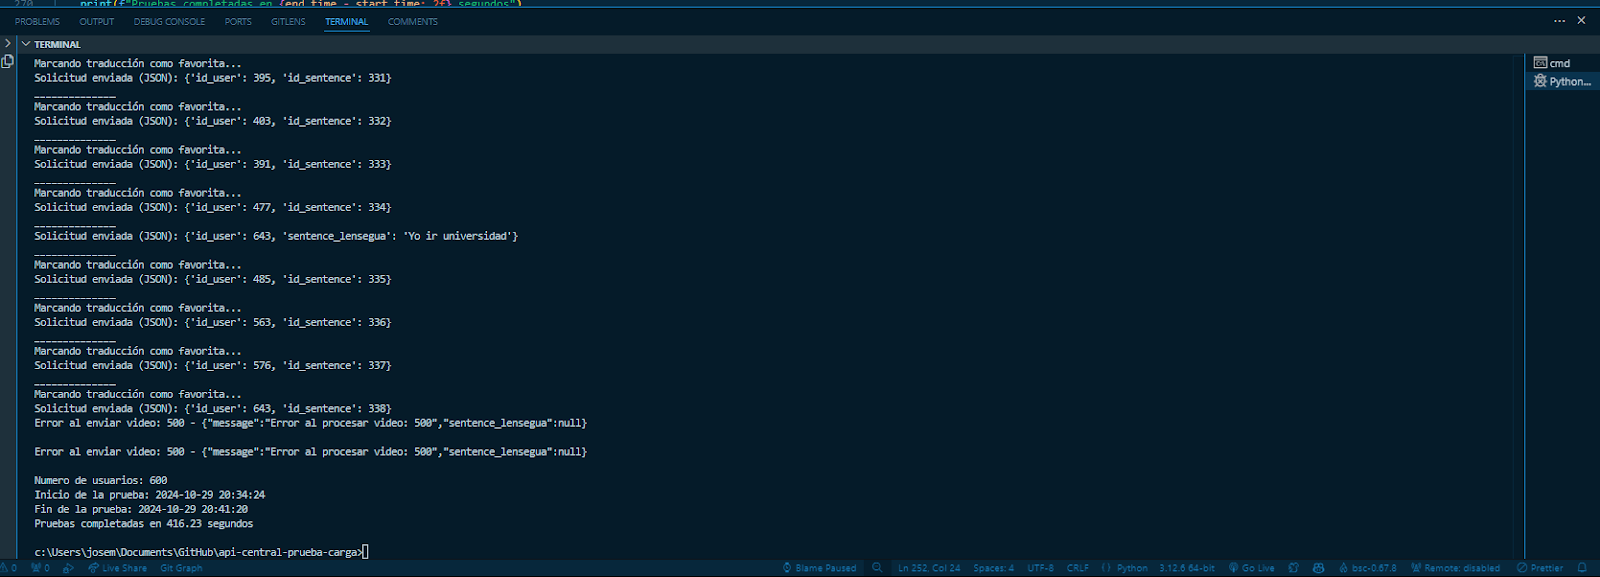
\includegraphics[width=0.5\textwidth]{figuras/pruebaCarga600U.png}
    \caption{Resultados de la prueba de carga con 600 usuarios concurrentes.}
    \label{fig:pruebaCarga600U}
\end{figure}

\begin{figure}[H]
    \centering
    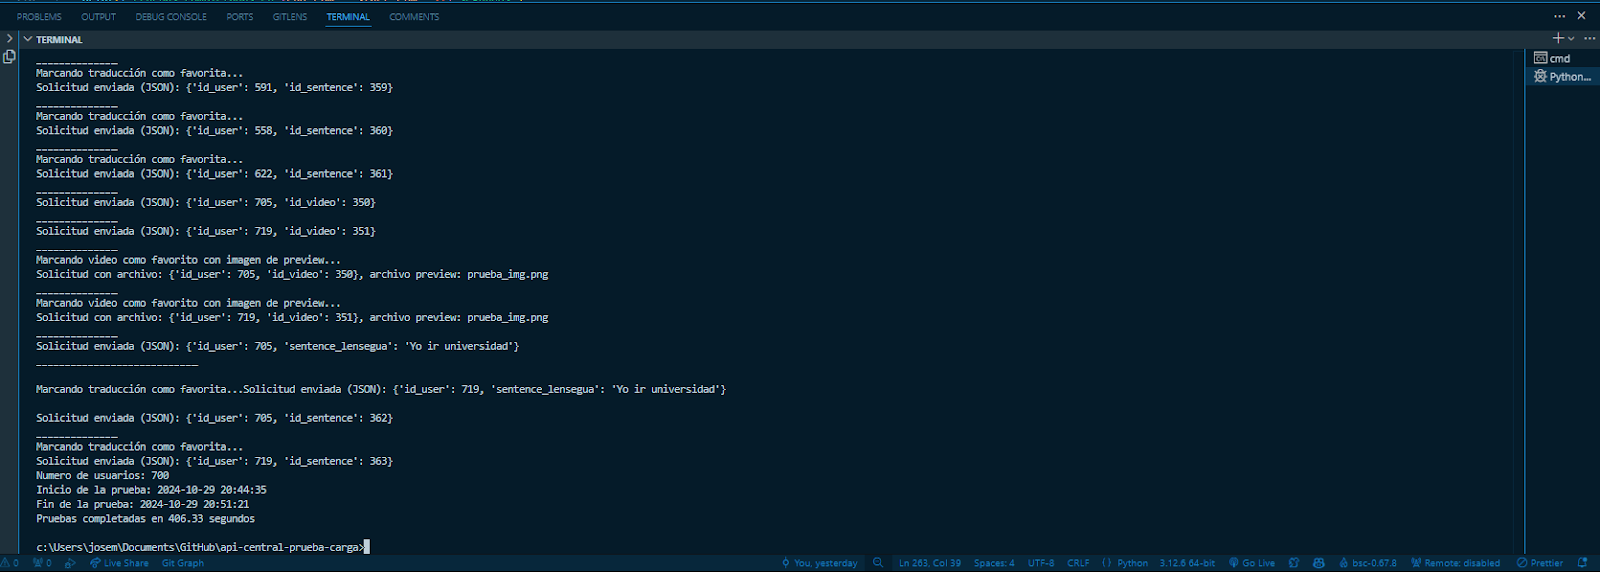
\includegraphics[width=0.5\textwidth]{figuras/pruebaCarga700U.png}
    \caption{Resultados de la prueba de carga con 700 usuarios concurrentes.}
    \label{fig:pruebaCarga700U}
\end{figure}

\begin{figure}[H]
    \centering
    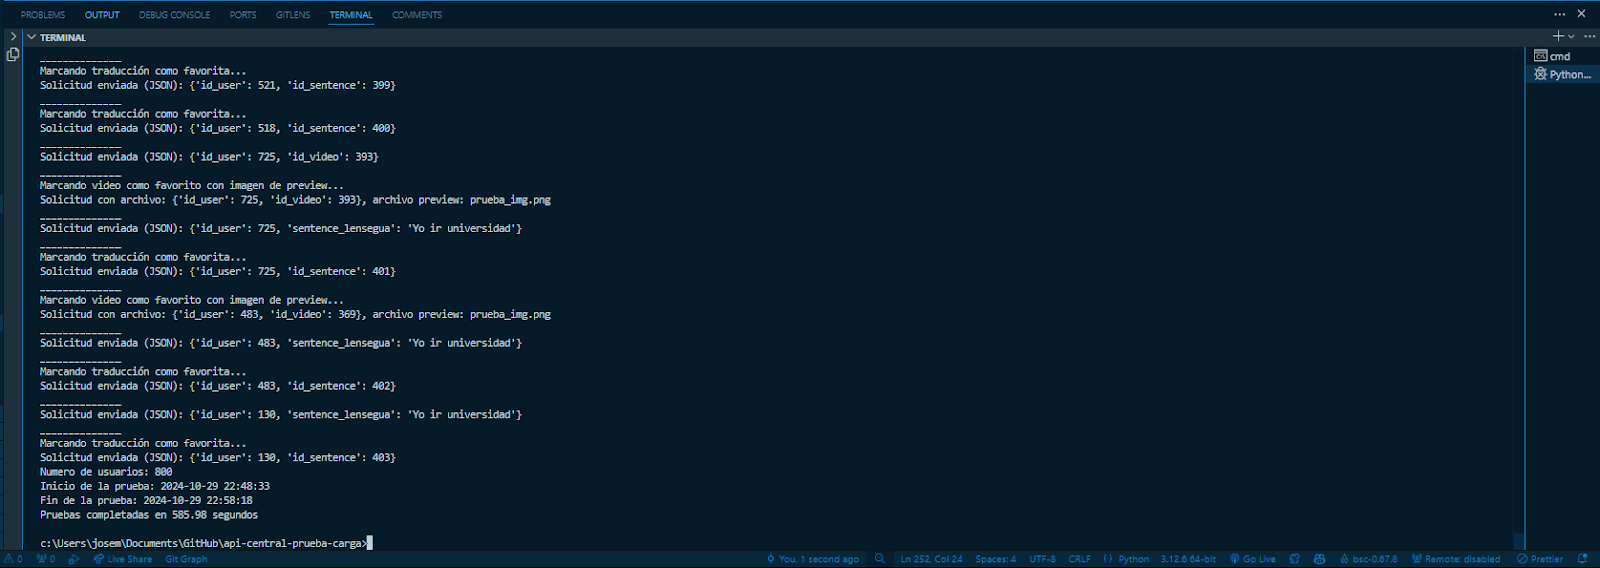
\includegraphics[width=0.5\textwidth]{figuras/pruebaCarga800U.png}
    \caption{Resultados de la prueba de carga con 800 usuarios concurrentes.}
    \label{fig:pruebaCarga800U}
\end{figure}

\begin{figure}[H]
    \centering
    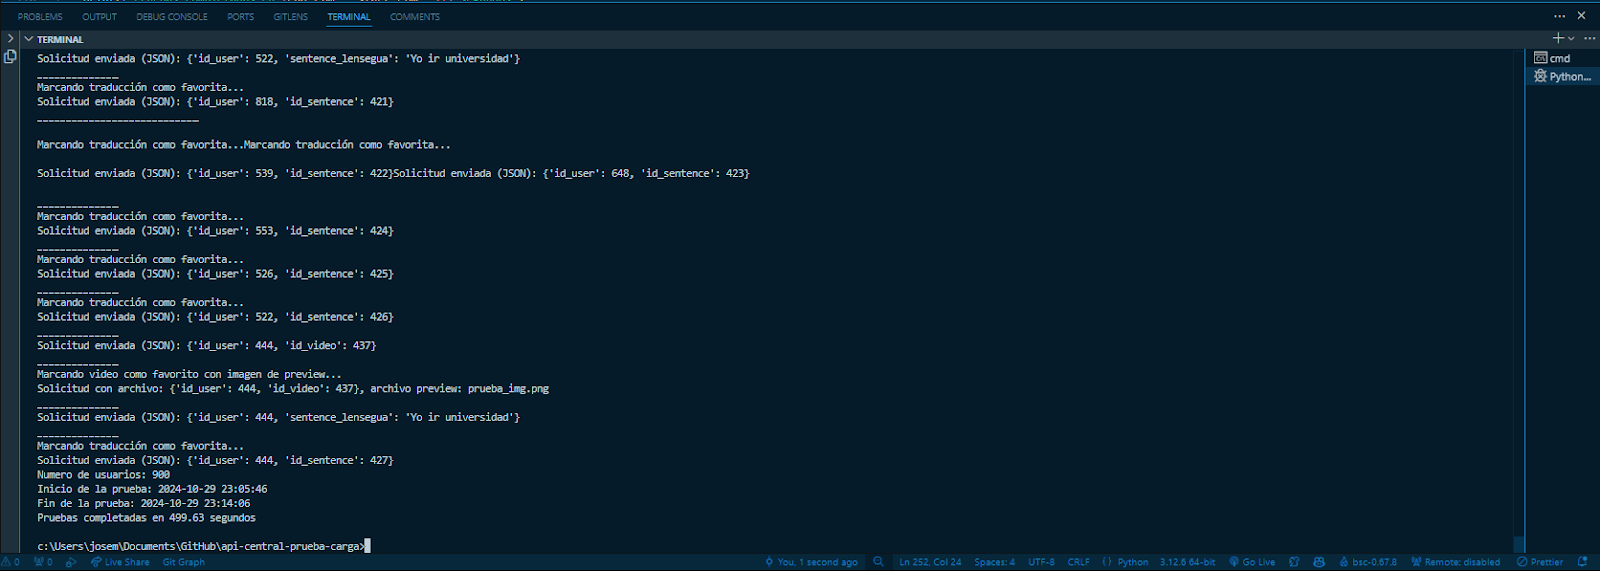
\includegraphics[width=0.5\textwidth]{figuras/pruebaCarga900U.png}
    \caption{Resultados de la prueba de carga con 900 usuarios concurrentes.}
    \label{fig:pruebaCarga900U}
\end{figure}

\begin{figure}[H]
    \centering
    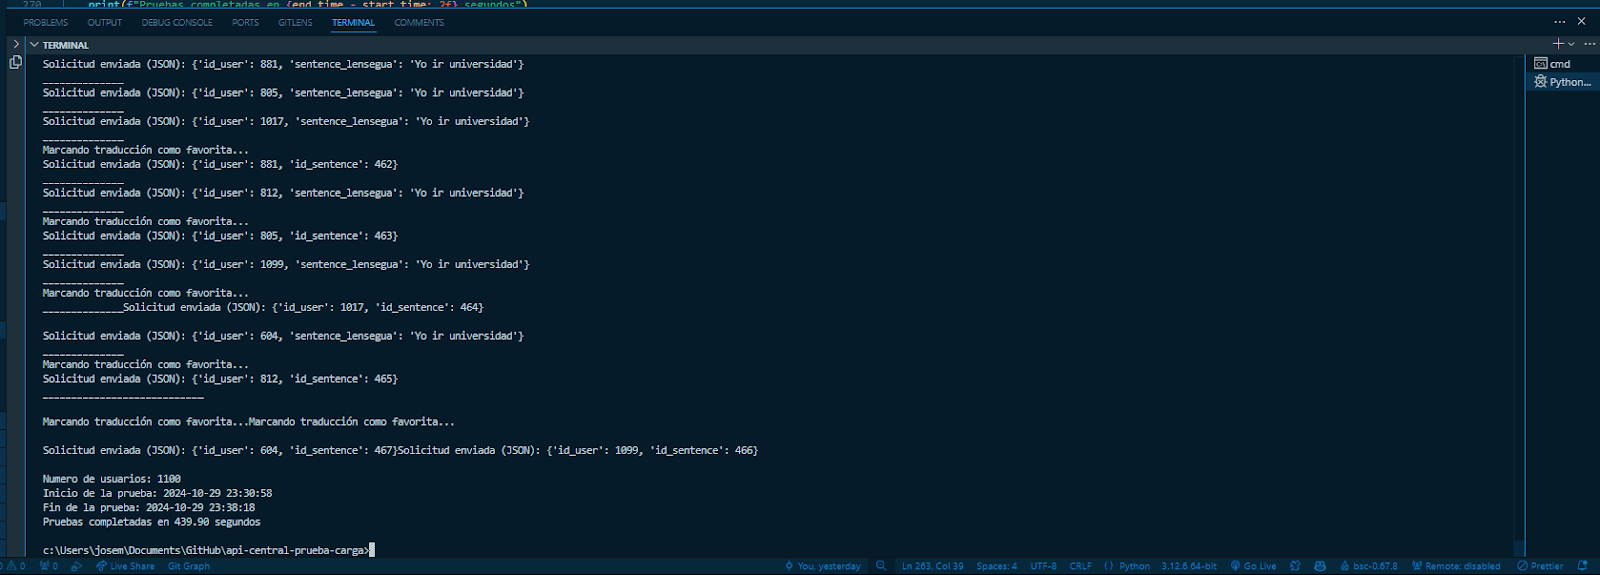
\includegraphics[width=0.5\textwidth]{figuras/pruebaCarga1100U.png}
    \caption{Resultados de la prueba de carga con 1100 usuarios concurrentes.}
    \label{fig:pruebaCarga1100U}
\end{figure}

\section{Pruebas de Extremo a Extremo (E2E)}

\subsection{Objetivo}
Las pruebas E2E validan el flujo completo de la aplicación desde la perspectiva del usuario, asegurando que todos los módulos y APIs se integren correctamente y que las funciones principales respondan adecuadamente en un flujo de uso continuo.

\subsection{Procedimiento}
\begin{enumerate}
    \item \textbf{Flujo Completo del Usuario}: Un usuario simulado realiza una serie de acciones que incluyen:
    \begin{itemize}
        \item Registro y autenticación.
        \item Acceso a su perfil, subida de video, marcación y eliminación de favoritos.
        \item Interacción con el sistema de traducciones y diccionario.
    \end{itemize}
    \item \textbf{Verificación y Tiempo de Respuesta}: Cada acción registra el tiempo de respuesta y verifica que el estado HTTP sea 200 (éxito). Esto garantiza que todas las funcionalidades respondan correctamente en un flujo integrado.
\end{enumerate}

% vamos a cargar la imagen e2e2test.png
La prueba End-to-End (E2E) se diseñó para evaluar el flujo completo de la aplicación desde la perspectiva del usuario, verificando que todas las APIs respondieran correctamente y que las funcionalidades se integraran de manera óptima. 

\section{Implementación de pruebas CVE para seguridad}

\begin{enumerate}
    \item \textbf{Identificación de Vulnerabilidades:}
    \begin{enumerate}
        \item Utilizar herramientas de escaneo de vulnerabilidades como Nessus, OpenVAS o Qualys para identificar posibles vulnerabilidades en el sistema.
        \item Asegurarse de que todas las vulnerabilidades identificadas estén referenciadas con sus respectivos identificadores CVE.
    \end{enumerate}
    
    \item \textbf{Evaluación de Vulnerabilidades:}
    \begin{enumerate}
        \item Realizar pruebas exhaustivas de seguridad para obtener los datos necesarios para la calculadora CVSS. Las pruebas incluyen:
        \begin{enumerate}
            \item Pruebas de Explotabilidad: Evaluar cuán fácilmente se puede explotar la vulnerabilidad, incluyendo factores como la complejidad del ataque y los privilegios requeridos.
            \item Pruebas de Impacto: Medir el impacto potencial de la vulnerabilidad en la confidencialidad, integridad y disponibilidad del sistema.
            \item Pruebas de Alcance: Determinar si la vulnerabilidad afecta sólo al componente vulnerable o si se puede propagar a otros componentes.
        \end{enumerate}
        \item Recopilar los datos obtenidos de las pruebas y utilizar una calculadora de puntaje CVE, como la proporcionada por el NVD (National Vulnerability Database), para calcular el puntaje de cada vulnerabilidad basada en los criterios de CVSS (Common Vulnerability Scoring System).
        \item \textbf{Criterios de CVSS:}
        \begin{enumerate}
            \item \textbf{Base Score}: Evaluación del impacto y la facilidad de explotación de la vulnerabilidad.
            \item \textbf{Temporal Score}: Considera factores temporales como la disponibilidad de explotaciones y parches.
            \item \textbf{Environmental Score}: Ajusta el puntaje base según el entorno y la configuración específicos.
        \end{enumerate}
    \end{enumerate}

    \item \textbf{Validación de Medidas de Seguridad:}
    \begin{enumerate}
        \item Implementar y validar las medidas de mitigación necesarias para corregir las vulnerabilidades identificadas.
        \item Realizar pruebas de validación post-mitigación para asegurar que las vulnerabilidades hayan sido corregidas y que las medidas no afecten negativamente el rendimiento del sistema.
    \end{enumerate}

    \item \textbf{Monitoreo Continuo:}
    \begin{enumerate}
        \item Realizar escaneos periódicos de vulnerabilidades para identificar nuevas amenazas y asegurarse de que las vulnerabilidades conocidas estén mitigadas.
        \item Recalcular los puntajes de CVE periódicamente para asegurar que el sistema se mantenga seguro.
    \end{enumerate}

    \item \textbf{Documentación y Reportes:}
    \begin{enumerate}
        \item Mantener un registro detallado de todas las vulnerabilidades identificadas, sus puntajes CVE y las acciones de mitigación realizadas.
        \item Generar reportes periódicos que incluyan análisis de tendencias en las vulnerabilidades y la efectividad de las medidas de seguridad implementadas.
    \end{enumerate}

    \item \textbf{Optimización y Mejora Continua:}
    \begin{enumerate}
        \item Basado en los análisis de vulnerabilidades y puntajes CVE, implementar ajustes necesarios en la configuración del servidor y las aplicaciones.
        \item Repetir las pruebas de seguridad para verificar las mejoras en la protección del sistema.
        \item Continuar el ciclo de pruebas y optimización hasta alcanzar un nivel óptimo de seguridad.
    \end{enumerate}
\end{enumerate}

\section{Pruebas de Seguridad con Lynis}

\subsection{Objetivo}
En este proyecto, se utilizó Lynis para auditar la seguridad del sistema mediante su Índice de Fortalecimiento. Este índice proporcionó una evaluación cuantitativa basada en la implementación de medidas de seguridad y prácticas recomendadas. Para cumplir con los objetivos del sistema, se definió una meta inicial de un puntaje de 40, considerado como la base para garantizar un sistema con medidas de seguridad básicas adecuadas. Este enfoque siguió las recomendaciones de la documentación de Lynis Hardening Index \cite{LynisHardeningIndex}, que establecía que un puntaje de 40 era suficiente para aplicaciones estándar, mientras que resultados más altos reflejaban un sistema más robusto. Según el CIS Benchmark \cite{CISBenchmarksReport}, una auditoría con un puntaje superior a 50 indicaba un fortalecimiento razonable para sistemas en entornos no críticos.

\subsection{Procedimiento}
\begin{enumerate}
    \item \textbf{Instalación y Ejecución}: Lynis fue instalado y ejecutado con el siguiente comando:
    \begin{verbatim}
    sudo lynis audit system
    \end{verbatim}
    Al finalizar, Lynis generó un informe con recomendaciones específicas para mejorar la seguridad del sistema.
    
    \item \textbf{Interpretación del Informe}: El informe proporcionado incluyó una puntuación general de seguridad, destacando las áreas de mayor riesgo y ofreciendo recomendaciones detalladas. 
\end{enumerate}

\section{Mejoras de Seguridad en \texttt{/etc/sysctl.conf}}

En base a las recomendaciones de Lynis, se realizaron ajustes en el archivo \texttt{/etc/sysctl.conf} para mejorar la seguridad de red del sistema. Estas configuraciones incluyen:

\begin{itemize}
    \item \textbf{Deshabilitar redirecciones ICMP} para prevenir ataques de red.
    \item \textbf{Habilitar SYN Cookies} para mitigar ataques SYN flood.
    \item \textbf{Restringir el uso de \texttt{dmesg} para usuarios no privilegiados}.
\end{itemize}

\section{Monitoreo Continuo de Seguridad con ClamAV}

\subsection{Instalación y Configuración}
ClamAV y su servicio de actualización \textbf{freshclam} fueron instalados para realizar escaneos de seguridad en el sistema de manera regular. Esto garantiza una capa adicional de protección contra amenazas de malware.

\subsection{Monitoreo y Ajustes Adicionales}
El sistema fue configurado para realizar escaneos periódicos y actualizar la base de datos de ClamAV. Esto permite mantener el sistema protegido frente a vulnerabilidades potenciales en el software o archivos nuevos.
